\documentclass[xcolor=dvipsnames]{beamer} 
\setbeamercolor{structure}{fg=OliveGreen!50!black} 
\usetheme{Madrid}
%\usetheme{CambridgeUS}
%\useoutertheme{tree}
%\usetheme{}
\usepackage{pgf,pgfarrows,pgfnodes,pgfautomata,pgfheaps}
\mode<handout>
{
	\usepackage{pgfpages}
	\pgfpagesuselayout{4 on 1}[a4paper,landscape,border shrink=5mm]
	%\pgfpagesuselayout{2 on 1}[a4paper,portrait,border shrink=5mm]
}
\usepackage{verbatim}
\usepackage{fancyhdr}
\usepackage{pstricks}
%\usepackage{beamerthemeiitb}
\usepackage{colortbl}
\usepackage{pst-node}
\usepackage{pst-grad}
\usepackage{pst-text}
\usepackage{pst-rel-points}
\usepackage{pst-coil}
\usepackage{amssymb}
%\usepackage{times}
\usepackage{calc}
\usepackage{etex}
\usepackage{ifthen}
%\usepackage{mydefs}
\usepackage{rotating}
\usepackage{multirow}
\usepackage{longtable}
\usepackage{color}
\usepackage[normalem]{ulem}
\usepackage{hyperref}
\usepackage{xspace}

\newcommand{\mustl}{\mbox{\sf MustL}}
\newcommand{\mustr}{\mbox{\sf MustR}}
\newcommand{\mustgen}{\mbox{\sf MustGen}}
\newcommand{\mustkill}{\mbox{\sf MustKill}}
\newcommand{\mustin}{\mbox{\sf MustIn}}
\newcommand{\mustout}{\mbox{\sf MustOut}}
\newcommand{\mayl}{\mbox{\sf MayL}}
\newcommand{\mayr}{\mbox{\sf MayR}}
\newcommand{\maygen}{\mbox{\sf MayGen}}
\newcommand{\maykill}{\mbox{\sf MayKill}}
\newcommand{\mayin}{\mbox{\sf MayIn}}
\newcommand{\mayout}{\mbox{\sf MayOut}}
%\newcommand{\In}[1]{\mbox{IN$_{#1}$}}
%\newcommand{\Out}[1]{\mbox{OUT$\!\!_{#1}$}}
\newcommand{\Gen}[1]{\mbox{Gen$_{#1}$}}
\newcommand{\Kill}[1]{\mbox{Kill$_{#1}$}}

\newcommand{\CPGEN}{\mbox{\sf CPGEN}}
\newcommand{\CPKILL}{\mbox{\sf CPKILL}}
\newcommand{\CPIN}{\mbox{\sf CPIN}}
\newcommand{\CPOUT}{\mbox{\sf CPOUT}}
\newcommand{\LHS}{\mbox{\sf LHS}}
\newcommand{\RHS}{\mbox{\sf\em RHS}}
\newcommand{\OPERANDS}{\mbox{\sf OPERANDS}}
\newcommand{\USE}{\mbox{\sf USE}}
\newcommand{\VARS}{\mbox{\sf VARS}}
\newcommand{\In}[1]{\mbox{\em In$_{#1}$}}
\newcommand{\Out}[1]{\mbox{\em Out$_{#1}$}}
\newcommand{\minus}{\ominus}
\newcommand{\RootVar}{\mbox{\sf\em Root\/}}
\newcommand{\clean}{\mbox{\sf\em CleanUp\/}}
\newcommand{\AP}[1]{\mbox{\sf\em P$\;({#1})$}}
\newcommand{\cupG}{{\;\uplus\;}}
\newcommand{\EFG}{\mbox{$\scalebox{1.2}{$\epsilon$}_{RG}$}}
\newcommand{\extend}[2]{\mbox{$#1\#\, #2$}}
\newcommand{\Empty}{\mbox{$\mathcal{E}$}}
\newcommand{\graphA}[1]{\text{{\sf\em makeGraph\/}$({#1})$}}
\newcommand{\graphO}[1]{\mbox{{\sf\em\small GOnly\/}$({#1})$}}
\newcommand{\Lin}[1]{\mbox{{\sf \em  ELIn}$_{#1}$}}
\newcommand{\Lout}[1]{\mbox{{\sf \em ELOut}$_{#1}$}}
\newcommand{\Lgen}[1]{\mbox{{\sf \em ELGen}$_{#1}$}}
\newcommand{\LgenC}[1]{\mbox{{\sf \em ELConstGen}$_{#1}$}}
\newcommand{\LgenT}[1]{\mbox{{\sf \em ELDepGen}$_{#1}$}}
\newcommand{\Lkill}[1]{\mbox{{\sf \em ELKillPath}$_{#1}$}}
\newcommand{\LLD}[1]{\mbox{\sf\em LDirect$_{#1}$}}
\newcommand{\LT}[1]{\mbox{\sf\em LTransfer$_{#1}$}}
\newcommand{\bigcupG}{{\biguplus}}


				 
\newcommand{\NULL}{\mbox{null\/}}
\newcommand{\undef}{\mbox{\sf\em undef\/}}
\newcommand{\nonconst}{\mbox{\sf\em nonconst\/}}
\newcommand{\Lt}{\mbox{$\widehat{L}\,$}}
\newcommand{\Ht}{\mbox{$\widehat{h}$}}
\newcommand{\Gt}{\mbox{$\widehat{g}$}}
\newcommand{\Xt}{\mbox{$\widehat{x}$}}
\newcommand{\Yt}{\mbox{$\widehat{y}$}}
\newcommand{\Bt}{\mbox{$\widehat{\bot}$}}
\newcommand{\Tt}{\mbox{$\widehat{\top}$}}
\newcommand{\HL}{\mbox{\bfseries\em H}}
\newcommand{\HT}{\mbox{$H$}}
\newcommand{\LD}{\mbox{$L$}}


\definecolor{blue}{named}{blue}
\definecolor{brown}{named}{brown}

\title{Incremental Data Flow analysis using PRISM}
\author[June'15]{Rashmi Rekha Mech \\
(\emph{Project Guide: Prof. Uday Khedker})}
\institute[IIT Bombay]{
\includegraphics{logo.eps}\\
Department of Computer Science and Engineering, \\ 
Indian Institute of Technology, Bombay}
%\titlegraphic{\scalebox{.9}{
\includegraphics{logo.eps}}}
\date[]{June 2015}

%%\hypersetup{
%%colorlinks=true,
%%linkcolor=brown
%%}
\definecolor{LightGreen}{rgb}{0.564706,0.933333,0.564706}
%%%%%%%%%%%%% Yellow
\newrgbcolor{yel}{0.95 1 .8}
\newcmykcolor{lightyellow}{0 0 .3 0}
\newcmykcolor{llyellow}{0 0 .2 .1}
%%%%%%%%%%%%% Green
\newrgbcolor{darkgreen}{0 .5 0}
\newrgbcolor{dgreen}{0 0.4 0}
%%%%%%%%%%%%% Gray
\newgray{lightgray}{.85}
\newgray{dgray}{.35}
\newgray{ldgray}{.75}
%%%%%%%%%%%%% Pink
\newcmykcolor{lpink}{0 .2 0 0}
\newrgbcolor{pink}{1 .5 .6}
%%%%%%%%%%%%% Magenta
\newcmykcolor{lmagenta}{0 .4 0 0}
%%%%%%%%%%%%% Blue
\newrgbcolor{oldlightblue}{.1 .85 1}
\newrgbcolor{lightblue}{.75 0.85 1}
\newrgbcolor{newlightblue}{.75 0.75 1}
\newrgbcolor{myblueother}{.5 .5 1}
\newrgbcolor{darkblue}{0 0 .5}
\newcmykcolor{llblue}{.2 .15 0 .1}
\newcmykcolor{lblue}{.3 .2 0 .1}
%%%%%%%%%%%%% Brown
\newrgbcolor{brown}{.65 0.15 .0}
%%%%%%%%%%%%% Cream
\newrgbcolor{cream}{.95 0.95 .65}
%%%%%%%%%%%%% Violet
\newrgbcolor{violet}{.84 0 .96}
\newrgbcolor{mygreen}{.24 .84 .72}
\newcommand{\irulethree}{\rule{0cm}{.3cm}}
\newcommand{\irulefour}{\rule{0cm}{.4cm}}
\newcommand{\irulefive}{\rule{0cm}{.5cm}}
\newcommand{\irulesix}{\rule{0cm}{.6cm}}


\newcommand{\lptr}{\mbox{\bfseries\footnotesize lptr}}
\newcommand{\rptr}{\mbox{\bfseries\footnotesize rptr}}
%\includeonlyframes{current}


\newcommand{\GenC}[1]{\mbox{{\sf\em ConstGen\/}$_{#1}$}}
\newcommand{\KillC}[1]{\mbox{{\sf\em ConstKill\/}$_{#1}$}}
\newcommand{\GenT}[1]{\mbox{{\sf\em DepGen\/}$_{#1}$}}
\newcommand{\KillT}[1]{\mbox{{\sf\em DepKill\/}$_{#1}$}}
\newcommand{\Cell}[3]{%

\psset{unit=5mm}

\begin{pspicture}(0,0)(6,4)
\psframe(0,0)(6.25,4)
\rput(4,2){\rnode{#1}{}}
\rput(2,2){#2}
\end{pspicture}
}
\newcommand{\Input}{\text{\sf\em input\/}\xspace}
\newcommand{\reachable}{\mbox{\sf\em reachable\/}}
\newcommand{\notReachable}{\mbox{\sf\em notReachable\/}}
\newcommand{\Start}[1]{\text{$\mbox{\sf\em Start}_{#1}$}}
\newcommand{\End}[1]{\text{$\mbox{\sf\em End}_{#1}$}}
\newcommand{\NEWMEETC}[2]{\text{\raisebox{-1.6ex}
                                {$\stackrel{#2}
                                {\stackrel{\bigersqcap_C}
                                        {\scriptstyle #1}}$}}}
\newcommand{\pred}{\text {\sf\em{pred}\/}}
\newcommand{\Succ}{\text{\sf\em {succ}\/}}
\newcommand{\bigersqcap}{{\psset{unit=1mm}%
			\begin{pspicture}(0,0)(3.5,4)
			\psline[linewidth=.3](0,0)(0,4)(3,4)(3,0)
                        \end{pspicture}
			}
                      }
\newcommand{\status}{\mbox{\sf\em status\/}}
\newcommand{\econd}{\mbox{\sf\em evalCond\/}}
\newcommand{\Undefined}{\mbox{\sf\em undefined\/}}
\newcommand{\etype}{\mbox{\sf\em label\/}}
\newcommand{\operands}{\ensuremath{\mbox{\sf\em Opd\/}}}
\newcommand{\ConstL}[1]{\mbox{{\sf\em ConstLeftL\/}$_{#1}$}}
\newcommand{\ConstR}[1]{\mbox{{\sf\em ConstRightL\/}$_{#1}$}}
\newcommand{\Const}{\mbox{\sf$\Bbb{C}$onst}}
\newcommand{\XD}{\text{$X$}}
\newcommand{\val}{\ensuremath{\mbox{\sf\em val\/}}}
\newcommand{\binop}{\ensuremath{\mbox{\sf\em bop\/}}}
\newcommand{\unop}{\ensuremath{\mbox{\sf\em uop\/}}}
\newcommand{\var}{\mbox{\sf$\Bbb{V}$ar}}
\newcommand{\gvar}{\mbox{\sf$\Bbb{G}$var}}
\newcommand{\lvar}{\mbox{\sf$\Bbb{L}$var}}
\newcommand{\expr}{\mbox{\sf$\Bbb{E}$xpr}}
\newcommand{\eval}{\ensuremath{\mbox{\sf\em eval\/}}}
\newcommand{\true}{\mbox{\sf\em true\/}}
\newcommand{\false}{\mbox{\sf\em false\/}}
\newcommand{\boundary}{\mbox{\sf\em BI}}

\newcommand{\NL}[1]{\hspace*{#1\TAL}}

\newlength{\codeLineLength}
\newcommand{\codeLine}[4]{#1 &
\psframebox[framesep=0,fillstyle=solid,fillcolor=#4,
	linestyle=none]{\makebox[\codeLineLength][l]{%
	\rule[-.3em]{0em}{.9em}{%
	 \NL{#2}{\mbox{#3}}}}}
\\ }
	


\newcommand{\Gax} % required
{\scalebox{.8}{
\large
{\psset{unit=.9mm}
\psset{linewidth=.3mm}
		\begin{pspicture}(-1,-3.5)(16,0)
%\psframe(-1,-2)(32,6)
		\psrelpoint{origin}{i}{8}{-2}
		\rput(\x{i},\y{i}){\rnode{i}{\pscirclebox[linestyle=none,fillstyle=solid,
				fillcolor=yellow,framesep=1.1]{$x$}}}
		\psrelpoint{origin}{j}{-1}{-2}
		\rput(\x{j},\y{j}){\rnode{j}{}}
		\ncline[linewidth=.4,doubleline=true]{->}{j}{i}
		\end{pspicture}
		}
}}

\newcommand{\Gbx} %required
{\scalebox{.8}{
\large
{\psset{unit=.9mm}
\psset{linewidth=.3mm}
		\begin{pspicture}(-1,-3.5)(35,0)
%\psframe(-1,-2)(32,6)
		\psrelpoint{origin}{i}{8}{-2}
		\rput(\x{i},\y{i}){\rnode{i}{\pscirclebox[linestyle=none,fillstyle=solid,
				fillcolor=yellow,framesep=1.1]{$x$}}}
		\psrelpoint{origin}{j}{-1}{-2}
		\rput(\x{j},\y{j}){\rnode{j}{}}
		\ncline[linewidth=.4,doubleline=true]{->}{j}{i}
		%%%%%%%%%%%%%%%%%%%%%%%%%%%%%%%%%%%%%%%%%%%%%%%%
		\psrelpoint{i}{m}{12}{0}
		\rput(\x{m},\y{m}){\rnode{m}{\pscirclebox[linestyle=none,fillstyle=solid,
				fillcolor=yellow,framesep=.5]{$l_4$}}}
		\ncline{->}{i}{m}
%		%\aput[0pt]{0}{$l$}
		%%%%%%%%%%%%%%%%%%%%%%%%%%%%%%%%%%%%%%%%%%%%%%%%
		\psrelpoint{m}{n}{12}{0}
		\rput(\x{n},\y{n}){\rnode{n}{\pscirclebox[linestyle=none,fillstyle=solid,
				fillcolor=yellow,framesep=.5]{$l_6$}}}
		\ncline{->}{m}{n}
		%\aput[0pt]{0}{$l$}
		\end{pspicture}
		}
}}

\newcommand{\Gcx}
{\scalebox{.8}{
\large
{\psset{unit=.9mm}
\psset{linewidth=.3mm}
		\begin{pspicture}(1,-8)(45,-3)
%\psframe(-1,-8)(42,1)
		\psrelpoint{origin}{k}{8}{-6}
		\rput(\x{k},\y{k}){\rnode{k}{\pscirclebox[linestyle=none,fillstyle=solid,
				fillcolor=yellow,framesep=1.1]{$x$}}}
		\psrelpoint{origin}{j}{-1}{-6}
		\rput(\x{j},\y{j}){\rnode{j}{}}
		\ncline[linewidth=.4,doubleline=true]{->}{j}{k}
		%%%%%%%%%%%%%%%%%%%%%%%%%%%%%%%%%%%%%%%%%%%%%%%%
		\psrelpoint{k}{l}{12}{0}
		\rput(\x{l},\y{l}){\rnode{l}{\pscirclebox[linestyle=none,fillstyle=solid,
				fillcolor=yellow,framesep=.6]{$r_3$}}}
		\ncline[nodesep=-.3]{->}{k}{l}
		%\aput[0pt]{0}{$r$}
		%%%%%%%%%%%%%%%%%%%%%%%%%%%%%%%%%%%%%%%%%%%%%%%%
		\psrelpoint{l}{m}{12}{0}
		\rput(\x{m},\y{m}){\rnode{m}{\pscirclebox[linestyle=none,fillstyle=solid,
				fillcolor=yellow,framesep=.5]{$l_4$}}}
		\ncline[nodesep=-.5]{->}{l}{m}
		%\aput[0pt]{0}{$l$}
		%%%%%%%%%%%%%%%%%%%%%%%%%%%%%%%%%%%%%%%%%%%%%%%%
		%\nccurve[angleA=-40,angleB=220,nodesep=-1]{->}{k}{m}
		%\ncline[nodesep=-.5]{->}{k}{m}
		%\bput[.5mm]{0}{$l$}
		%\nccurve[angleA=45,angleB=135,nodesep=-1,ncurv=1.8]{->}{l}{l}
		%\nccurve[angleA=-45,angleB=-135,nodesep=-1,ncurv=.5]{->}{k}{m}
		\psrelpoint{m}{n}{12}{0}
		\rput(\x{n},\y{n}){\rnode{n}{\pscirclebox[linestyle=none,fillstyle=solid,
				fillcolor=yellow,framesep=.5]{$l_6$}}}
		\ncline[nodesep=-.5]{->}{m}{n}
		%\aput[0pt]{0}{$l$}
		\end{pspicture}
		}
}
}
\newcommand{\Gdx}
{\scalebox{.75}{
\large
{\psset{unit=.9mm}
\psset{linewidth=.3mm}
		\begin{pspicture}(-1,-9)(45,-3)
%\psframe(-1,-8)(42,1)
		\psrelpoint{origin}{k}{8}{-6}
		\rput(\x{k},\y{k}){\rnode{k}{\pscirclebox[linestyle=none,fillstyle=solid,
				fillcolor=yellow,framesep=1.1]{$x$}}}
		\psrelpoint{origin}{j}{-1}{-6}
		\rput(\x{j},\y{j}){\rnode{j}{}}
		\ncline[linewidth=.4,doubleline=true]{->}{j}{k}
		%%%%%%%%%%%%%%%%%%%%%%%%%%%%%%%%%%%%%%%%%%%%%%%%
		\psrelpoint{k}{l}{12}{0}
		\rput(\x{l},\y{l}){\rnode{l}{\pscirclebox[linestyle=none,fillstyle=solid,
				fillcolor=yellow,framesep=.6]{$r_3$}}}
		\ncline[nodesep=-.3]{->}{k}{l}
		%\aput[0pt]{0}{$r$}
		%%%%%%%%%%%%%%%%%%%%%%%%%%%%%%%%%%%%%%%%%%%%%%%%
		\psrelpoint{l}{m}{12}{0}
		\rput(\x{m},\y{m}){\rnode{m}{\pscirclebox[linestyle=none,fillstyle=solid,
				fillcolor=yellow,framesep=.5]{$l_4$}}}
		\ncline[nodesep=-.5]{->}{l}{m}
		%\aput[0pt]{0}{$l$}
		%%%%%%%%%%%%%%%%%%%%%%%%%%%%%%%%%%%%%%%%%%%%%%%%
		%\nccurve[angleA=-40,angleB=220,nodesep=-1]{->}{k}{m}
		%\ncline[nodesep=-.5]{->}{k}{m}
		%\bput[.5mm]{0}{$l$}
		%\nccurve[angleA=45,angleB=135,nodesep=-1,ncurv=1.8]{->}{l}{l}
		\nccurve[angleA=-45,angleB=-135,nodesep=-1,ncurv=.5]{->}{k}{m}
		\psrelpoint{m}{n}{12}{0}
		\rput(\x{n},\y{n}){\rnode{n}{\pscirclebox[linestyle=none,fillstyle=solid,
				fillcolor=yellow,framesep=.5]{$l_6$}}}
		\ncline[nodesep=-.5]{->}{m}{n}
		%\aput[0pt]{0}{$l$}
		\end{pspicture}
		}
}
}
\newcommand{\Gex} % required
{\scalebox{.75}{
\large
{\psset{unit=.9mm}
\psset{linewidth=.3mm}
		\begin{pspicture}(1,-9)(45,-2)
%\psframe(-1,-8)(42,1)
		\psrelpoint{origin}{k}{8}{-6}
		\rput(\x{k},\y{k}){\rnode{k}{\pscirclebox[linestyle=none,fillstyle=solid,
				fillcolor=yellow,framesep=1.1]{$x$}}}
		\psrelpoint{origin}{j}{-1}{-6}
		\rput(\x{j},\y{j}){\rnode{j}{}}
		\ncline[linewidth=.4,doubleline=true]{->}{j}{k}
		%%%%%%%%%%%%%%%%%%%%%%%%%%%%%%%%%%%%%%%%%%%%%%%%
		\psrelpoint{k}{l}{12}{0}
		\rput(\x{l},\y{l}){\rnode{l}{\pscirclebox[linestyle=none,fillstyle=solid,
				fillcolor=yellow,framesep=.6]{$r_3$}}}
		\ncline[nodesep=-.3]{->}{k}{l}
		%\aput[0pt]{0}{$r$}
		%%%%%%%%%%%%%%%%%%%%%%%%%%%%%%%%%%%%%%%%%%%%%%%%
		\psrelpoint{l}{m}{12}{0}
		\rput(\x{m},\y{m}){\rnode{m}{\pscirclebox[linestyle=none,fillstyle=solid,
				fillcolor=yellow,framesep=.5]{$l_4$}}}
		\ncline[nodesep=-.5]{->}{l}{m}
		%\aput[0pt]{0}{$l$}
		%%%%%%%%%%%%%%%%%%%%%%%%%%%%%%%%%%%%%%%%%%%%%%%%
		%\nccurve[angleA=-40,angleB=220,nodesep=-1]{->}{k}{m}
		%\ncline[nodesep=-.5]{->}{k}{m}
		%\bput[.5mm]{0}{$l$}
		\nccurve[angleA=45,angleB=135,nodesep=-1,ncurv=1.8]{->}{l}{l}
		\nccurve[angleA=-45,angleB=-135,nodesep=-1,ncurv=.5]{->}{k}{m}
		\psrelpoint{m}{n}{12}{0}
		\rput(\x{n},\y{n}){\rnode{n}{\pscirclebox[linestyle=none,fillstyle=solid,
				fillcolor=yellow,framesep=.5]{$l_6$}}}
		\ncline[nodesep=-.5]{->}{m}{n}
		%\aput[0pt]{0}{$l$}
		\end{pspicture}
		}
}
}
\newcommand{\Ggx} % required
{\scalebox{.75}{
\large
{\psset{unit=.9mm}
\psset{linewidth=.3mm}
		\begin{pspicture}(1,-9)(45,-2)
%\psframe(-1,-8)(42,1)
		\psrelpoint{origin}{k}{8}{-6}
		\rput(\x{k},\y{k}){\rnode{k}{\pscirclebox[linestyle=none,fillstyle=solid,
				fillcolor=yellow,framesep=1.1]{$x$}}}
		\psrelpoint{origin}{j}{-1}{-6}
		\rput(\x{j},\y{j}){\rnode{j}{}}
		\ncline[linewidth=.4,doubleline=true]{->}{j}{k}
		%%%%%%%%%%%%%%%%%%%%%%%%%%%%%%%%%%%%%%%%%%%%%%%%
		\psrelpoint{k}{l}{12}{0}
		\rput(\x{l},\y{l}){\rnode{l}{\pscirclebox[linestyle=none,fillstyle=solid,
				fillcolor=yellow,framesep=.6]{$r_3$}}}
		\ncline[nodesep=-.3]{->}{k}{l}
		%\aput[0pt]{0}{$r$}
		%%%%%%%%%%%%%%%%%%%%%%%%%%%%%%%%%%%%%%%%%%%%%%%%
		\psrelpoint{l}{m}{12}{0}
		\rput(\x{m},\y{m}){\rnode{m}{\pscirclebox[linestyle=none,fillstyle=solid,
				fillcolor=yellow,framesep=.5]{$l_4$}}}
		\ncline[nodesep=-.5]{->}{l}{m}
		%\aput[0pt]{0}{$l$}
		%%%%%%%%%%%%%%%%%%%%%%%%%%%%%%%%%%%%%%%%%%%%%%%%
		%\nccurve[angleA=-40,angleB=220,nodesep=-1]{->}{k}{m}
		%\ncline[nodesep=-.5]{->}{k}{m}
		%\bput[.5mm]{0}{$l$}
		\nccurve[angleA=45,angleB=135,nodesep=-1,ncurv=1.8]{->}{l}{l}
		%\nccurve[angleA=-45,angleB=-135,nodesep=-1,ncurv=.5]{->}{k}{m}
		\psrelpoint{m}{n}{12}{0}
		\rput(\x{n},\y{n}){\rnode{n}{\pscirclebox[linestyle=none,fillstyle=solid,
				fillcolor=yellow,framesep=.5]{$l_6$}}}
		\ncline[nodesep=-.5]{->}{m}{n}
		%\aput[0pt]{0}{$l$}
		\end{pspicture}
		}
}
}
\newcommand{\Gay} % required
{\scalebox{.8}{
\large
{\psset{unit=.9mm}
\psset{linewidth=.3mm}
		\begin{pspicture}(5,-3.5)(12,0)
%\psframe(-1,-2)(32,6)
		\psrelpoint{origin}{i}{8}{-2}
		\rput(\x{i},\y{i}){\rnode{i}{\pscirclebox[linestyle=none,fillstyle=solid,
				fillcolor=yellow,framesep=1.1]{$y$}}}
		\psrelpoint{origin}{j}{-1}{-2}
		\rput(\x{j},\y{j}){\rnode{j}{}}
		\ncline[linewidth=.4,doubleline=true]{->}{j}{i}
		%%%%%%%%%%%%%%%%%%%%%%%%%%%%%%%%%%%%%%%%%%%%%%%%
		%\psrelpoint{i}{m}{10}{0}
		%\rput(\x{m},\y{m}){\rnode{m}{\pscirclebox[framesep=.5]{$l_5$}}}
		%\ncline{->}{i}{m}
		%%\aput[0pt]{0}{$l$}
		%%%%%%%%%%%%%%%%%%%%%%%%%%%%%%%%%%%%%%%%%%%%%%%%
		%\psrelpoint{i}{n}{10}{0}
		%\rput(\x{n},\y{n}){\rnode{n}{\pscirclebox[framesep=.5]{$l_7$}}}
		%\ncline{->}{i}{n}
		%%\aput[0pt]{0}{$l$}
		\end{pspicture}
		}
}}

\newcommand{\Gby} %required
{\scalebox{.8}{
\large
{\psset{unit=.9mm}
\psset{linewidth=.3mm}
		\begin{pspicture}(5,-3.5)(23,0)
%\psframe(-1,-2)(32,6)
		\psrelpoint{origin}{i}{8}{-2}
		\rput(\x{i},\y{i}){\rnode{i}{\pscirclebox[linestyle=none,fillstyle=solid,
				fillcolor=yellow,framesep=1.1]{$y$}}}
		\psrelpoint{origin}{j}{-1}{-2}
		\rput(\x{j},\y{j}){\rnode{j}{}}
		\ncline[linewidth=.4,doubleline=true]{->}{j}{i}
		%%%%%%%%%%%%%%%%%%%%%%%%%%%%%%%%%%%%%%%%%%%%%%%%
		%\psrelpoint{i}{m}{12}{0}
		%\rput(\x{m},\y{m}){\rnode{m}{\pscirclebox[framesep=.5]{$l_5$}}}
		%\ncline{->}{i}{m}
		%\aput[0pt]{0}{$l$}
		%%%%%%%%%%%%%%%%%%%%%%%%%%%%%%%%%%%%%%%%%%%%%%%%
		\psrelpoint{i}{n}{12}{0}
		\rput(\x{n},\y{n}){\rnode{n}{\pscirclebox[linestyle=none,fillstyle=solid,
				fillcolor=yellow,framesep=.5]{$l_6$}}}
		\ncline{->}{i}{n}
		%\aput[0pt]{0}{$l$}
		\end{pspicture}
		}
}}
\newcommand{\Gaz} % required
{\scalebox{.85}{
\large
{\psset{unit=.9mm}
\psset{linewidth=.3mm}
		\begin{pspicture}(0,-3.5)(10,0)
%\psframe(-1,-2)(32,6)
		\psrelpoint{origin}{i}{8}{-2}
		\rput(\x{i},\y{i}){\rnode{i}{\pscirclebox[linestyle=none,fillstyle=solid,
				fillcolor=yellow,framesep=1.1]{$z$}}}
		\psrelpoint{origin}{j}{-1}{-2}
		\rput(\x{j},\y{j}){\rnode{j}{}}
		\ncline[linewidth=.4,doubleline=true]{->}{j}{i}
		%%%%%%%%%%%%%%%%%%%%%%%%%%%%%%%%%%%%%%%%%%%%%%%%
		%\psrelpoint{i}{m}{12}{0}
		%\rput(\x{m},\y{m}){\rnode{m}{\pscirclebox[framesep=.5]{$l_5$}}}
		%\ncline{->}{i}{m}
		%%\aput[0pt]{0}{$l$}
		%%%%%%%%%%%%%%%%%%%%%%%%%%%%%%%%%%%%%%%%%%%%%%%%
		%\psrelpoint{i}{n}{12}{0}
		%\rput(\x{n},\y{n}){\rnode{n}{\pscirclebox[framesep=.5]{$l_7$}}}
		%\ncline{->}{i}{n}
		%\aput[0pt]{0}{$l$}
		\end{pspicture}
		}
}}

\psset{unit=1mm}
\newcommand{\memGraph}{%
\begin{pspicture}(0,0)(38,20)
\psframe(0,0)(38,20)
%\psframe[linestyle=none,fillstyle=solid,fillcolor=lightyellow](12,0)(40,50)
%\psframe[linestyle=none,fillstyle=solid,fillcolor=lightyellow](0,0)(10,50)
\putnode{n0}{origin}{2}{16}{\pscirclebox[linestyle=none]{$x$}}
\putnode{n1}{n0}{0}{-12}{\pscirclebox[linestyle=none]{$y$}}
\putnode{n01}{n0}{10}{0}{\pscirclebox[framesep=2.8]{}}
\putnode{n11}{n1}{10}{0}{\pscirclebox[framesep=2.8]{}}
\putnode{n3}{n01}{10}{-6}{\pscirclebox[framesep=2.8]{}}
\putnode{n4}{n3}{12}{0}{\pscirclebox[framesep=2.8]{}}
%
\ncline[nodesepA=-.5]{->}{n0}{n01}
\ncline[nodesepA=-.6]{->}{n1}{n11}
\ncline[nodesep=-.5]{->}{n01}{n3}
\aput[2pt](.5){$l$}
\ncline[nodesep=-.5]{->}{n11}{n3}
\bput[2pt](.5){$r$}
\ncline{->}{n3}{n4}
\aput[2pt](.5){$n$}
\end{pspicture}
}
%\setbeamertemplate{frametitle}[default][center]
%\setbeamerfont{page number in head/foot}{size=\tiny}
%\setbeamertemplate{headline}[frame number]
%\usetheme{CambridgeUS}    
%\usecolortheme[named=Green]{structure} 
%\usetheme{Boadilla}


\begin{document}

\frame[plain]{\titlepage}

\frame{
\frametitle{Outline of the talk}
\begin{itemize}
  \item Incremental Data Flow analysis
  \begin{itemize}
  \item Bit-vector frameworks
  \item General frameworks
  \item Method to reduce the size of affected region
  \end{itemize}
  \item Overview of PRISM 
  \item Incremental driver
  \begin{itemize}
    \item Testing
   \end{itemize}
  \item Limitations of old Solver
  \item Future work
\end{itemize}
}

\part{Incremental Data Flow Analysis}
\frame{\partpage}

\frame{
\frametitle{Why Incremental Analysis?}
When program undergoes changes:
\begin{itemize}
 \item Some or all computed data flow information become invalid
 \item Re-computation is required
\end{itemize}
}

\frame{
\frametitle{Motivating Example - Available Expression Analysis}
\begin{pspicture}(0,0)(100,80)
% \psframe(0,0)(100,90)
\onslide<1->
\putnode{n1}{origin}{60}{70}{%
     \psframebox[linewidth=.3,framesep=0.3]{\begin{tabular}{c} $a*b$ \\ $b+d$
                                             
                                            \end{tabular}
}}
\putnode{a}{n1}{-13}{0}{n1}
\putnode{n2}{n1}{0}{-15}{%
     \psframebox[linewidth=.3,framesep=1.5]{$a+b$}}
\putnode{b}{n2}{10}{0}{n2}
\putnode{n3}{n2}{-20}{-13}{%
     \psframebox[linewidth=.3,framesep=1.5]{$b+d$}}
\putnode{c}{n3}{-10}{0}{n3}
\putnode{n4}{n3}{0}{-15}{%
     \psframebox[linewidth=.3,framesep=0.3]{\begin{tabular}{c} $a=1$ \\ $a+b$
                                             \end{tabular}
}}
\putnode{d}{n4}{-12}{0}{n4}
\putnode{n5}{n2}{20}{-20}{%
     \psframebox[linewidth=.3,framesep=1.5]{$d=1$}}
\putnode{e}{n5}{-10}{0}{n5}
\putnode{n6}{n5}{0}{-15}{%
     \psframebox[linewidth=.3,framesep=1.5]{$a+b$}}
\putnode{f}{n6}{-10}{0}{n6}

\putnode{n7}{n6}{0}{-15}{%
   \psframebox[linewidth=.3,framesep=0.7]{%
   \begin{tabular}{c|c|c}
			$a*b$ & $b+d$ & $a+b$\\
			\end{tabular}}}
\putnode{n8}{n7}{-30}{0}{Bit Vector}

\ncline{->}{n1}{n2}
\ncline{->}{n2}{n3}
\ncline{->}{n2}{n5}
\ncline{->}{n3}{n4}
\ncloop[armA=3,armB=3,angleA=-90,angleB=90,loopsize=19,
		linearc=1,offsetB=1]{->}{n4}{n3}
\ncloop[armA=3,armB=3,angleA=-90,angleB=90,loopsize=-10,
		linearc=0.8,offsetB=1, offsetA=2]{->}{n5}{n2}
\ncline{->}{n5}{n6}

\onslide<2-7>
\putnode{g}{n1}{-40}{8}{1st Iteration}

\onslide<3->
\putnode{g}{n1}{-12}{5}{\blue$\langle000\rangle$}

\onslide<4->
\putnode{g}{n1}{-12}{-5}{\blue$\langle110\rangle$}

\onslide<5-7>
\putnode{g}{n2}{-10}{4}{\blue$\langle110\rangle$}

\onslide<6-7>
\putnode{g}{n2}{-10}{-4}{\blue$\langle111\rangle$}
\putnode{g}{n5}{-10}{4}{\blue$\langle111\rangle$}

\onslide<6-8>
\putnode{g}{n3}{-10}{4}{\blue$\langle111\rangle$}

\onslide<8->
\putnode{g}{n1}{-40}{8}{2nd Iteration}

\onslide<7-8>
\putnode{g}{n3}{-10}{-4}{\blue$\langle111\rangle$}
\putnode{g}{n4}{-12}{5}{\blue$\langle111\rangle$}
\putnode{g}{n4}{-12}{-5}{\blue$\langle011\rangle$}
\putnode{g}{n5}{-10}{-4}{\blue$\langle101\rangle$}
\putnode{g}{n6}{-10}{4}{\blue$\langle101\rangle$}
\putnode{g}{n6}{-10}{-4}{\blue$\langle101\rangle$}

\onslide<8->
\putnode{g}{n2}{-10}{4}{\red$\langle100\rangle$}
\putnode{g}{n2}{-10}{-4}{\red$\langle101\rangle$}
% \putnode{g}{n3}{-10}{4}{\red$\langle101\rangle$}
\putnode{g}{n5}{-10}{4}{\red$\langle101\rangle$}

\onslide<9->
\putnode{g}{n3}{-10}{4}{\red$\langle001\rangle$}
\putnode{g}{n3}{-10}{-4}{\red$\langle001\rangle$}
\putnode{g}{n4}{-12}{5}{\red$\langle001\rangle$}
\putnode{g}{n4}{-12}{-5}{\blue$\langle011\rangle$}
\putnode{g}{n6}{-10}{4}{\blue$\langle101\rangle$}
\putnode{g}{n6}{-10}{-4}{\blue$\langle101\rangle$}
\putnode{g}{n5}{-10}{-4}{\blue$\langle101\rangle$}

\end{pspicture}
}

\frame{ 
\frametitle{Motivating Example - Available Expression Analysis}
\begin{itemize}
 \item It requires 3 iterations to converge
\end{itemize}
}

\frame{
\frametitle{Motivating Example - Available Expression Analysis }
\begin{pspicture}(0,0)(100,80)
% \psframe(0,0)(100,90)
\onslide<1->
\putnode{n1}{origin}{40}{70}{%
     \psframebox[linewidth=.3,framesep=0.3]{\begin{tabular}{c} $a*b$ \\ $b+d$
                                             
                                            \end{tabular}
}}
\putnode{a}{n1}{-13}{0}{n1}
\putnode{n2}{n1}{0}{-15}{%
     \psframebox[linewidth=.3,framesep=1.5]{$a+b$}}
\putnode{b}{n2}{10}{0}{n2}
\putnode{n3}{n2}{-20}{-13}{%
     \psframebox[linewidth=.3,framesep=1.5]{$b+d$}}
\putnode{c}{n3}{-10}{0}{n3}
\putnode{n4}{n3}{0}{-15}{%
     \psframebox[linewidth=.3,framesep=0.3]{\begin{tabular}{c} $a=1$ \\ $a+b$
                                             \end{tabular}
}}
\putnode{d}{n4}{-12}{0}{n4}
\putnode{n5}{n2}{20}{-20}{%
     \psframebox[linewidth=.3,framesep=1.5]{$d=1$}}
\putnode{e}{n5}{-10}{0}{n5}
\putnode{n6}{n5}{0}{-15}{%
     \psframebox[linewidth=.3,framesep=2.5]{\hspace{10mm}}}
\putnode{x}{n6}{0}{0}{$a+b$}
\putnode{f}{n6}{-10}{0}{n6}

\putnode{n7}{n6}{0}{-15}{%
   \psframebox[linewidth=.3,framesep=0.7]{%
   \begin{tabular}{c|c|c}
			$a*b$ & $b+d$ & $a+b$\\
			\end{tabular}}}
\putnode{n8}{n7}{-30}{0}{Bit Vector}

\ncline{->}{n1}{n2}
\ncline{->}{n2}{n3}
\ncline{->}{n2}{n5}
\ncline{->}{n3}{n4}
\ncloop[armA=3,armB=3,angleA=-90,angleB=90,loopsize=19,
		linearc=1,offsetB=1]{->}{n4}{n3}
\ncloop[armA=3,armB=3,angleA=-90,angleB=90,loopsize=-10,
		linearc=0.8,offsetB=1, offsetA=2]{->}{n5}{n2}
\ncline{->}{n5}{n6}

\onslide<2->
\putnode{x}{n6}{0}{0}{\red \sout{$a+b$}}
 \onslide<3->
\putnode{g}{n1}{-12}{5}{\blue$\langle000\rangle$}
\putnode{g}{n1}{-12}{-5}{\blue$\langle110\rangle$}
\putnode{g}{n2}{-10}{4}{\blue$\langle100\rangle$}
\putnode{g}{n2}{-10}{-4}{\blue$\langle101\rangle$}
\putnode{g}{n5}{-10}{4}{\blue$\langle101\rangle$}
\putnode{g}{n3}{-10}{4}{\blue$\langle001\rangle$}
\putnode{g}{n3}{-10}{-4}{\blue$\langle001\rangle$}
\putnode{g}{n4}{-12}{5}{\blue$\langle001\rangle$}
\putnode{g}{n4}{-12}{-5}{\blue$\langle011\rangle$}
\putnode{g}{n5}{-10}{-4}{\blue$\langle101\rangle$}
\putnode{g}{n6}{-10}{4}{\blue$\langle101\rangle$}
\putnode{g}{n6}{-10}{-4}{\blue$\langle101\rangle$}

\putnode{h}{n1}{45}{0}{\red No Change in data flow values}

\end{pspicture}
}

\frame{ 
\frametitle{Motivating Example - Available Expression Analysis}
\begin{itemize}
 \item Recomputing the values from the scratch is very inefficient 
 \item Need an incremental analysis:
      \begin{itemize}
       \item modifies only affected data flow information
       \item more cost effective then \textbf{exhaustive} analysis
      \end{itemize}
\end{itemize}
}


\part{Incremental Analysis in Bit-vector Framework}
\frame{\partpage}


\frame{
\frametitle{Flow functions in bit-vector frameworks}
\begin{itemize}
 \item Possible flow functions:
	\begin{itemize}
	 \item Raise : Result is always top
	 \item Lower : Result is always bottom
	 \item Propagate : Propagates the value from one program point to another
	\end{itemize}
\end{itemize}
}

\frame{ 
\frametitle{Example for Flow Functions}
\begin{pspicture}(0,0)(0,50)
%%\psframe(0,0)(50,50)
\onslide<1->
 \putnode{n1}{origin}{35}{40}{%
      \psframebox[linewidth=.3,framesep=2.5, framearc=.4]{\hspace{10mm}}}
%  \onslide<1->
\putnode{a0}{n1}{30}{20}{\textbf{Available Expression Analysis}}
\putnode{a}{n1}{-10}{0}{n1}
\putnode{n2}{n1}{0}{-15}{%
     \psframebox[linewidth=.3,framesep=2.5, framearc=.4]{\hspace{10mm}}}
\putnode{n3}{n2}{0}{-15}{%
     \psframebox[linewidth=.3,framesep=2.5, framearc=.4]{\hspace{10mm}}}

\putnode{a}{n3}{-10}{0}{n3}
% \putnode{a1}{n3}{0}{-10}{(a)}
 \ncline{->}{n1}{n2}
\ncline{->}{n2}{n3}

\onslide<1-3>
\putnode{a}{n2}{-10}{0}{n2}

\onslide<1-1>
\putnode{z}{n1}{0}{0}{$a*b$}

\onslide<1-5>
 \putnode{z1}{n3}{0}{0}{$b=1$}

\onslide<2-3>
\putnode{a1}{n1}{40}{0}{\textbf{Raise Function}}
\putnode{z}{n1}{0}{0}{\red$a*b$}
\putnode{a2}{a1}{10}{-15}{\begin{tabular}{l}
                         Gen$_1 = 1$\\
                         Kill$_1 = 0$ \\
                         IN$_1 = 0$ \\
                         OUT$_1 = $Gen$_1 \cup$ (IN$_1$-Kill$_1$)  = 1\\
                        \end{tabular}
}

\onslide<3-3>
\putnode{b}{a1}{0}{-30}{\red Result is always top}

\onslide<3->
\putnode{z}{n1}{0}{0}{$a*b$}

\onslide<4-5>
\putnode{a1}{n1}{40}{0}{\textbf{Propagate Function}}
\putnode{a}{n2}{-10}{0}{\red n2}	
\putnode{a2}{a1}{10}{-15}{\begin{tabular}{l}
                         Gen$_2 = 0$\\
                         Kill$_2 = 0$ \\
                         IN$_2 = 1$ \\
                         OUT$_2 = $Gen$_2 \cup$ (IN$_2$-Kill$_2$) = IN$_2$ = 1\\
                        \end{tabular}
}

\onslide<5-5>
\putnode{b}{a1}{10}{-30}{\red Propagates the value at IN to OUT}
 
\onslide<6->
\putnode{a}{n2}{-10}{0}{n2}
\putnode{z1}{n3}{0}{0}{\red$b=1$}
\putnode{a1}{n1}{40}{0}{\textbf{Lower Function}}
\putnode{a2}{a1}{10}{-15}{\begin{tabular}{l}
                         Gen$_3 = 0$\\
                         Kill$_3 = 1$ \\
                         IN$_3 = 1$ \\
                         OUT$_3 = $Gen$_3 \cup$ (IN$_3$-Kill$_3$) = 0\\
                        \end{tabular}
}

\onslide<7->
\putnode{b}{a1}{10}{-30}{\red Result is always bottom}


\end{pspicture}
}

\frame{ 
\frametitle{Changes in Bit-vector Frameworks}
\begin{itemize}
 \item As a consequence of some change in a node, some data flow values may:
      \begin{itemize}
       \item change from top to bottom
       \item change from bottom to top
       \item remain same
      \end{itemize}
\end{itemize}
}

\frame{ 
\frametitle{Possible Changes in Flow Functions for Top to Bottom Change}
\begin{pspicture}(0,10)(0,40)
%%\psframe(0,0)(50,50)
\putnode{n1}{origin}{45}{30}{%
     \psframebox[linewidth=.3,framesep=2.5]{raise}}
 \putnode{a}{n1}{0}{10}{\textit{old}}
\putnode{n2}{n1}{0}{-15}{%
     \psframebox[linewidth=.3,framesep=2.5]{propagate}}
%  \putnode{a}{n2}{-10}{0}{n2}


\putnode{n12}{n1}{30}{0}{%
     \psframebox[linewidth=.3,framesep=2.5]{lower}}
 \putnode{a}{n12}{0}{10}{\textit{new}}
\putnode{n22}{n12}{0}{-15}{%
     \psframebox[linewidth=.3,framesep=2.5]{propagate}}
% \putnode{a}{n22}{-10}{0}{n2}
% \putnode{a1}{n2}{15}{-10}{(a)}
\ncline{->}{n1}{n12}
\ncline{->}{n1}{n22}
\ncline{->}{n2}{n12}

\psline[linestyle=dotted](60,40)(60,10)

\end{pspicture}
}

\frame{ 
\frametitle{Possible Changes in Flow Functions for Top to Bottom Change}
\begin{pspicture}(0,10)(0,40)
\putnode{n1}{origin}{45}{30}{%
     \psframebox[linewidth=.3,framesep=2.5]{lower}}
 \putnode{a}{n1}{0}{10}{\textit{old}}
\putnode{n2}{n1}{0}{-15}{%
     \psframebox[linewidth=.3,framesep=2.5]{propagate}}
%  \putnode{a}{n2}{-10}{0}{n2}


\putnode{n12}{n1}{30}{0}{%
     \psframebox[linewidth=.3,framesep=2.5]{raise}}
 \putnode{a}{n12}{0}{10}{\textit{new}}
\putnode{n22}{n12}{0}{-15}{%
     \psframebox[linewidth=.3,framesep=2.5]{propagate}}
% \putnode{a}{n22}{-10}{0}{n2}
% \putnode{a1}{n2}{15}{-10}{(b)}
\ncline{->}{n1}{n12}
\ncline{->}{n1}{n22}
\ncline{->}{n2}{n12}

\psline[linestyle=dotted](60,40)(60,10)
\end{pspicture}
}

\frame{ 
\frametitle{Handling Top to Bottom Change}
\begin{itemize}
 \item Top value is an intermediate value until data flow analysis is completed
 \item Whenever there is top to bottom change, the changes can be propagated directly to its neighbouring nodes
\end{itemize}
}


\frame{
\frametitle{Example for Top to Bottom Change}
\begin{pspicture}(0,0)(50,50)
%%\psframe(0,0)(50,50)
\onslide<1->
\putnode{n1}{origin}{55}{40}{%
     \psframebox[linewidth=.3,framesep=2.5, framearc=.4]{$b*c$}}
\putnode{a}{n1}{-10}{0}{n1}
\putnode{n2}{n1}{0}{-15}{%
     \psframebox[linewidth=.3,framesep=2.5, framearc=.4]{\hspace{10mm}}}
\putnode{b}{n2}{-11}{0}{n2}
\putnode{n3}{n2}{0}{-15}{%
      \psframebox[linewidth=.3,framesep=2.5, framearc=.4]{\hspace{10mm}}}
\putnode{c}{n3}{-10}{0}{n3}
\ncline{->}{n1}{n2}
\ncline{->}{n2}{n3}
\ncloop[armA=3,armB=3,angleA=-90,angleB=90,loopsize=-17,
		linearc=0.5,offsetB=1]{->}{n3}{n2}
\onslide<1-4>
\putnode{a}{n3}{0}{0}{$b*c$}

\onslide<1-4>
\putnode{x}{n1}{5}{17}{\blue Initial Available Expression Analysis}
		
\onslide<2-5>
\putnode{d}{n1}{-8}{4}{\blue0}
\putnode{d}{n1}{-8}{-4}{\blue1}
\putnode{e}{n3}{-8}{-4}{\blue1}

\onslide<3-5>
\putnode{f}{n2}{-8}{4}{\blue1}

\onslide<4-5>
\putnode{f}{n2}{-8}{-4}{\blue1}
\putnode{e}{n3}{-8}{4}{\blue1}

\onslide<5-5>
% \putnode{d}{n1}{-3}{-6}{\red1}
\putnode{a}{n3}{0}{0}{\red \sout{$b*c$}}

\onslide<6->
\putnode{a}{n3}{0}{0}{\red$b=$}
\putnode{x}{n1}{5}{17}{\blue Top to Bottom change}
\putnode{d}{n1}{-8}{4}{\lightblue0}
\putnode{d}{n1}{-8}{-4}{\lightblue1}
\putnode{e}{n3}{-8}{-4}{\lightblue1}
\putnode{f}{n2}{-8}{4}{\lightblue1}
\putnode{f}{n2}{-8}{-4}{\lightblue1}
\putnode{e}{n3}{-8}{4}{\lightblue1}
\putnode{w}{n2}{30}{0}{ \psframebox[linewidth=.3,framesep=1.5, framearc=.4]{Raise}}
\putnode{y}{w}{25}{0}{ \psframebox[linewidth=.3,framesep=1.5, framearc=.4]{Lower}}
\ncline{->}{w}{y}

\onslide<7->
\putnode{d}{n1}{8}{-4}{\blue1}
\putnode{e}{n3}{8}{-4}{\red0}
\putnode{x}{n1}{40}{0}{\red IN$_2$=OUT$_1 \cap$ OUT$_3$}
\putnode{x1}{n3}{5}{-15}{\red Directly Propagate the change to its neighbour}
\onslide<8->
\putnode{f}{n2}{8}{4}{\red0}

\onslide<9->
\putnode{f}{n2}{8}{-4}{\red0}
\putnode{e}{n3}{8}{4}{\red0}
\end{pspicture}
}

\frame{ 
\frametitle{Handling Bottom to Top Change}
\begin{itemize}
 \item Bottom value is a final value even during analysis
 \item Whenever there is bottom to top change, we cannot directly propagate the changes to its neighbouring nodes
 \item Need some more processing
\end{itemize}
}

\frame{
\frametitle{Example for Bottom to Top Change}
\begin{pspicture}(0,0)(50,50)
%%\psframe(0,0)(50,50)
\onslide<1->
\putnode{n1}{origin}{55}{40}{%
     \psframebox[linewidth=.3,framesep=2.5, framearc=.4]{$b=$}}
\putnode{a}{n1}{-10}{0}{n1}
\putnode{n2}{n1}{0}{-15}{%
     \psframebox[linewidth=.3,framesep=2.5, framearc=.4]{\hspace{10mm}}}
\putnode{b}{n2}{-11}{0}{n2}
\putnode{n3}{n2}{0}{-15}{%
      \psframebox[linewidth=.3,framesep=2.5, framearc=.4]{\hspace{10mm}}}
\putnode{c}{n3}{-10}{0}{n3}
\ncline{->}{n1}{n2}
\ncline{->}{n2}{n3}
\ncloop[armA=3,armB=3,angleA=-90,angleB=90,loopsize=-17,
		linearc=0.5,offsetB=1]{->}{n3}{n2}
\onslide<1-4>
\putnode{a}{n3}{0}{0}{$b=$}
\onslide<1-4>
\putnode{x}{n1}{5}{17}{\blue Initial Available Expression Analysis}		
		
\onslide<2-4>
\putnode{d}{n1}{-8}{4}{\blue0}
\putnode{d}{n1}{-8}{-4}{\blue0}
\putnode{e}{n3}{-8}{-4}{\blue0}
% \putnode{d}{n1}{-3}{-6}{\red0}
% \putnode{e}{n3}{-3}{-6}{\red0}

\onslide<3-4>
\putnode{f}{n2}{-8}{4}{\blue0}
% \putnode{f}{n2}{-3}{5}{\red0}

\onslide<4-4>
\putnode{f}{n2}{-8}{-4}{\blue0}
\putnode{e}{n3}{-8}{4}{\blue0}
% \putnode{f}{n2}{-3}{-5}{\red0}
% \putnode{e}{n3}{-3}{6}{\red0}

\onslide<5-5>
% \putnode{d}{n1}{-3}{-6}{\red1}
\putnode{a}{n3}{0}{0}{\red\sout{$b=$}}

\onslide<6->
\putnode{x}{n1}{5}{17}{\blue Bottom to Top change}
\putnode{a}{n3}{0}{0}{\red$b*c$}
\putnode{d}{n1}{-8}{4}{\lightblue0}
\putnode{d}{n1}{-8}{-4}{\lightblue0}
\putnode{e}{n3}{-8}{-4}{\lightblue0}
\putnode{f}{n2}{-8}{4}{\lightblue0}
\putnode{f}{n2}{-8}{-4}{\lightblue0}
\putnode{e}{n3}{-8}{4}{\lightblue0}
\putnode{w}{n2}{30}{0}{ \psframebox[linewidth=.3,framesep=1.5, framearc=.4]{Lower}}
\putnode{y}{w}{25}{0}{ \psframebox[linewidth=.3,framesep=1.5, framearc=.4]{Raise}}
\ncline{->}{w}{y}



\onslide<7->
\putnode{d}{n1}{8}{-4}{\blue0}
\putnode{e}{n3}{8}{-4}{\red1}
\putnode{x}{n1}{40}{0}{\red IN$_2$=OUT$_1 \cap$ OUT$_3$}
\putnode{x1}{n3}{0}{-15}{\blue Cannot propagate the change to its neighbouring nodes}

\onslide<8->
\putnode{d}{n1}{8}{-4}{\blue0}
\putnode{f}{n2}{8}{4}{\red0}

\onslide<9->
\putnode{f}{n2}{8}{-4}{\red0}
\putnode{e}{n3}{8}{4}{\red0}
\end{pspicture}
}

\frame{ 
\frametitle{Bottom to Top Change}
\begin{itemize}
 \item Need some more processing
\end{itemize}
}

\frame{ 
\frametitle{Bottom to Top Change}
\begin{itemize}
 \onslide<1->
 \item Steps to incorporate bottom to top change:
 \begin{itemize}
 \onslide<2->
  \item Identify the data flow values which may become top
  \onslide<3->
  \item Find out the data flow values which must remain bottom due to the effect of some other property
 \end{itemize}

\end{itemize}
}

\frame{
\frametitle{Motivating Example}
\begin{pspicture}(0,0)(100,90)
%%\psframe(0,0)(100,90)
\onslide<1->
\putnode{n1}{origin}{25}{80}{%
     \psframebox[linewidth=.3,framesep=1.7]{ $a+b$}}
\putnode{a}{n1}{-10}{0}{n1}

\putnode{n2}{n1}{0}{-15}{%
     \psframebox[linewidth=.3,framesep=1.7]{$a*b$}}
\putnode{b}{n2}{-10}{0}{n2}

\putnode{n3}{n2}{-20}{-15}{%
     \psframebox[linewidth=.3,framesep=2.7]{\hspace{10mm}}}

\putnode{c}{n3}{10}{0}{n3}

\putnode{n4}{n2}{20}{-15}{%
     \psframebox[linewidth=.3,framesep=2.5]{\hspace{10mm}}}
\putnode{d}{n4}{-10}{0}{n4}

\putnode{n5}{n2}{0}{-30}{%
     \psframebox[linewidth=.3,framesep=1.7]{$a*c$}}
\putnode{e}{n5}{-9}{0}{n5}

\putnode{n6}{n5}{0}{-15}{%
     \psframebox[linewidth=.3,framesep=2.5]{\hspace{10mm}}}
\putnode{f}{n6}{-10}{0}{n6}
\putnode{g}{n6}{40}{-7}{%
     \psframebox[linewidth=.3,framesep=0.7]{\begin{tabular}{c|c|c}
			  $a+b$ & $a*b$ & $a*c$\\                          
                          \end{tabular}}}
\ncline{->}{n1}{n2}
\ncline{->}{n2}{n3}
\ncline{->}{n3}{n5}
\ncline{->}{n2}{n4}
\ncline{->}{n4}{n5}
\ncline{->}{n5}{n6}
\ncloop[armA=3,armB=3,angleA=-90,angleB=90,loopsize=-30,
		linearc=0.5,offsetA=2, offsetB=2]{->}{n5}{n2}
\onslide<1-2>
\putnode{x}{n3}{0}{0}{$b=2$}

\onslide<2->
\putnode{h}{n1}{65}{0}{Initial Available Expression Analysis}
\putnode{x1}{n1}{-10}{5}{\blue$\langle000\rangle$}
\putnode{x1}{n1}{-10}{-5}{\blue$\langle100\rangle$}
\putnode{x1}{n2}{-10}{5}{\blue$\langle000\rangle$}
\putnode{x1}{n2}{0}{-5}{\blue$\langle010\rangle$}
\putnode{x1}{n3}{0}{5}{\blue$\langle010\rangle$}
\putnode{x1}{n3}{0}{-5}{\blue$\langle000\rangle$}
\putnode{x1}{n4}{0}{5}{\blue$\langle010\rangle$}
\putnode{x1}{n4}{0}{-5}{\blue$\langle010\rangle$}
\putnode{x1}{n5}{-11}{3}{\blue$\langle000\rangle$}
\putnode{x1}{n5}{-10}{-5}{\blue$\langle001\rangle$}
\putnode{x1}{n6}{-10}{5}{\blue$\langle001\rangle$}
\putnode{x1}{n6}{-10}{-5}{\blue$\langle001\rangle$}




\onslide<2-3>
\putnode{i}{h}{3}{-25}{\begin{tabular}{c c c c c c c}
			\hline
			& \multicolumn{2}{c}{$a+b$} & \multicolumn{2}{c}{$a*b$} & \multicolumn{2}{c}{$a*c$} \\
			\hline
			Node & In & Out & In & Out & In & Out\\
			\hline
			1. & 0 & 1 & 0 & 0 & 0 & 0 \\
			2. & 0 & 0 & 0 & 1 & 0 & 0 \\
			3. & 0 & 0 & 1 & 0 & 0 & 0 \\
			4. & 0 & 0 & 1 & 1 & 0 & 0 \\
			5. & 0 & 0 & 0 & 0 & 0 & 1 \\
			6. & 0 & 0 & 0 & 0 & 1 & 1\\
			\hline
			\end{tabular}}
		
\onslide<3->
\putnode{x}{n3}{0}{0}{\red\sout{$b=2$}}
	
\onslide<4->
\putnode{j}{n1}{50}{-30}{ \psframebox[linewidth=.3,framesep=0.7]{lower}}
\putnode{k}{j}{30}{0}{ \psframebox[linewidth=.3,framesep=0.7]{propagate}}

\onslide<5->
\ncline{->}{j}{k}

\onslide<6->
\putnode{l}{k}{-15}{-10}{\red Bottom to top change}

\end{pspicture}
}

\frame{
\frametitle{Motivating Example - Step 1}
\begin{itemize}
 \item The data flow values which were 0 and \textit{may} become 1 due to this change
 \begin{itemize}
 \item <2->Affected region
 \end{itemize}
\end{itemize}
}

\frame{
 \frametitle{Motivating Example - Step 1}
\begin{pspicture}(0,0)(100,90)
%%\psframe(0,0)(100,90)
\onslide<1->
\putnode{n1}{origin}{25}{80}{%
     \psframebox[linewidth=.3,framesep=1.7]{ $a+b$}}
\putnode{a}{n1}{-10}{0}{n1}

\putnode{n2}{n1}{0}{-15}{%
     \psframebox[linewidth=.3,framesep=1.7]{$a*b$}}


\putnode{n3}{n2}{-20}{-15}{%
     \psframebox[linewidth=.3,framesep=2.7]{\hspace{10mm}}}



\putnode{n4}{n2}{20}{-15}{%
     \psframebox[linewidth=.3,framesep=2.5]{\hspace{10mm}}}


\putnode{n5}{n2}{0}{-30}{%
     \psframebox[linewidth=.3,framesep=1.7]{$a*c$}}


\putnode{n6}{n5}{0}{-15}{%
     \psframebox[linewidth=.3,framesep=2.5]{\hspace{10mm}}}

\putnode{g}{n6}{40}{-7}{%
     \psframebox[linewidth=.3,framesep=0.7]{\begin{tabular}{c|c|c}
			  $a+b$ & $a*b$ & $a*c$\\                          
                          \end{tabular}}}
\ncline{->}{n1}{n2}
\ncline{->}{n2}{n3}
\ncline{->}{n3}{n5}
\ncline{->}{n2}{n4}
\ncline{->}{n4}{n5}
\ncline{->}{n5}{n6}
\ncloop[armA=3,armB=3,angleA=-90,angleB=90,loopsize=-30,
		linearc=0.5,offsetA=2, offsetB=2]{->}{n5}{n2}


\onslide<1->
\putnode{x}{n3}{0}{0}{\red\sout{$b=2$}}

\onslide<1-2>
\putnode{b}{n2}{-10}{0}{n2}
\putnode{c}{n3}{10}{0}{n3}
\putnode{d}{n4}{-10}{0}{n4}
\putnode{e}{n5}{-9}{0}{n5}
\putnode{f}{n6}{-10}{0}{n6}

\onslide<2->
\putnode{c}{n3}{10}{0}{\red n3}
\putnode{e}{n5}{-9}{0}{\red n5}
\putnode{f}{n6}{-10}{0}{\red n6}

\onslide<3->
\putnode{b}{n2}{-10}{0}{\red n2}
\putnode{d}{n4}{-10}{0}{n4}
\onslide<3->
\putnode{d}{n4}{-10}{0}{\red n4}

\onslide<3-3>
\putnode{h}{n1}{65}{-20}{Affected Region}
\putnode{i}{h}{3}{-10}{\begin{tabular}{c} \red $\langle$ OUT$_3 ,$ IN$_5 ,$ OUT$_5 ,$ IN$_6 ,$ OUT$_6 ,$ \\ \red IN$_2 ,$ OUT$_2,$ IN$_4,$ OUT$_4,$ IN$_3 \rangle$
                        \end{tabular}}
		
\onslide<4->
\putnode{h}{n1}{65}{-10}{\blue Data flow values which may become 1}

\onslide<1-11>		
\putnode{x1}{n1}{-10}{5}{\blue$\langle000\rangle$}
\putnode{x1}{n1}{-10}{-5}{\blue$\langle100\rangle$}

\onslide<1-6>\putnode{x1}{n2}{-10}{5}{$\langle$\blue000$\rangle$}
\onslide<1-7>\putnode{x1}{n2}{0}{-5}{$\langle$\blue010$\rangle$}
\onslide<1-8>\putnode{x1}{n3}{0}{5}{\blue$\langle$010$\rangle$}
\onslide<1-3>\putnode{x1}{n3}{0}{-5}{$\langle$\blue000$\rangle$}
\onslide<1-8>\putnode{x1}{n4}{0}{5}{$\langle$\blue010$\rangle$}
\onslide<1-9>\putnode{x1}{n4}{0}{-5}{$\langle$\blue010$\rangle$}
\onslide<1-4>\putnode{x1}{n5}{-11}{3}{$\langle$\blue000$\rangle$}
\onslide<1-5>\putnode{x1}{n5}{-10}{-5}{$\langle$\blue001$\rangle$}
\onslide<1-6>\putnode{x1}{n6}{-10}{5}{$\langle$\blue001$\rangle$}
\onslide<1-6>\putnode{x1}{n6}{-10}{-5}{$\langle$\blue001$\rangle$}


\onslide<7-10>\putnode{x1}{n2}{-10}{5}{$\langle$\red00\blue0$\rangle$}
\onslide<8-10>\putnode{x1}{n2}{0}{-5}{$\langle$\red0\blue10$\rangle$}
\onslide<9-10>\putnode{x1}{n3}{0}{5}{\blue$\langle$\red0\blue10$\rangle$}
\onslide<4-10>\putnode{x1}{n3}{0}{-5}{$\langle$\red00\blue0$\rangle$}
\onslide<9-10>\putnode{x1}{n4}{0}{5}{$\langle$\red0\blue10$\rangle$}
\onslide<10-10>\putnode{x1}{n4}{0}{-5}{$\langle$\red0\blue10$\rangle$}
\onslide<5-10>\putnode{x1}{n5}{-11}{3}{$\langle$\red00\blue0$\rangle$}
\onslide<6-10>\putnode{x1}{n5}{-10}{-5}{$\langle$\red00\blue1$\rangle$}
\onslide<7-10>\putnode{x1}{n6}{-10}{5}{$\langle$\red00\blue1$\rangle$}
\onslide<7-10>\putnode{x1}{n6}{-10}{-5}{$\langle$\red00\blue1$\rangle$}

\onslide<11->
\putnode{i}{h}{3}{-25}{\begin{tabular}{c c c c c c c }
    \hline
       & \multicolumn{2}{c}{$a+b$} & \multicolumn{2}{c}{$a*b$} & \multicolumn{2}{c}{$a*c$} \\
    \hline
      Node & In & Out & In & Out & In & Out\\
   	\hline
   	  1. &  &  &  &  &  &  \\
   	  2. & 1 & 1 & 1 &  &  &  \\
   	  3. & 1 & 1 &  & 1 &  &  \\
   	  4. & 1 & 1 &  &  &  &  \\
   	  5. & 1 & 1 & 1 & 1 &  &  \\
   	  6. & 1 & 1 & 1 & 1 &  & \\
      
      \hline
    \end{tabular}}

    
\putnode{x1}{n1}{-10}{5}{\blue$\langle000\rangle$}
\putnode{x1}{n1}{-10}{-5}{\blue$\langle100\rangle$}
\putnode{x1}{n2}{-10}{5}{$\langle$\red11\blue0$\rangle$}
\putnode{x1}{n2}{0}{-5}{$\langle$\red1\blue10$\rangle$}
\putnode{x1}{n3}{0}{5}{\blue$\langle$\red1\blue10$\rangle$}
\putnode{x1}{n3}{0}{-5}{$\langle$\red11\blue0$\rangle$}
\putnode{x1}{n4}{0}{5}{$\langle$\red1\blue10$\rangle$}
\putnode{x1}{n4}{0}{-5}{$\langle$\red1\blue10$\rangle$}
\putnode{x1}{n5}{-11}{3}{$\langle$\red11\blue0$\rangle$}
\putnode{x1}{n5}{-10}{-5}{$\langle$\red11\blue1$\rangle$}
\putnode{x1}{n6}{-10}{5}{$\langle$\red11\blue1$\rangle$}
\putnode{x1}{n6}{-10}{-5}{$\langle$\red11\blue1$\rangle$}
    
    % \putnode{x}{n3}{0}{0}{\red$b=2$}
		
\end{pspicture}
}

\frame{
\frametitle{Motivating Example - Step 2}
\begin{itemize}
 \item Find out the data flow values which must remain bottom due to the effect of some other property
 \begin{itemize}
 \item<2-> Initialize affected region to top.
 \item<3-> Identify boundary nodes
 \item<4-> Compute values at boundary nodes and propagate them
 \end{itemize}
\end{itemize}
}


\frame{
 \frametitle{Motivating Example - Step 2}
\begin{pspicture}(0,0)(100,90)
%%\psframe(0,0)(100,90)
\onslide<1->
\putnode{n1}{origin}{25}{80}{%
     \psframebox[linewidth=.3,framesep=1.7]{ $a+b$}}
\putnode{a}{n1}{-10}{0}{n1}

\putnode{n2}{n1}{0}{-15}{%
     \psframebox[linewidth=.3,framesep=1.7]{$a*b$}}


\putnode{n3}{n2}{-20}{-15}{%
     \psframebox[linewidth=.3,framesep=2.7]{\hspace{10mm}}}



\putnode{n4}{n2}{20}{-15}{%
     \psframebox[linewidth=.3,framesep=2.5]{\hspace{10mm}}}


\putnode{n5}{n2}{0}{-30}{%
     \psframebox[linewidth=.3,framesep=1.7]{$a*c$}}


\putnode{n6}{n5}{0}{-15}{%
     \psframebox[linewidth=.3,framesep=2.5]{\hspace{10mm}}}

\putnode{g}{n6}{40}{-7}{%
     \psframebox[linewidth=.3,framesep=0.7]{\begin{tabular}{c|c|c}
			  $a+b$ & $a*b$ & $a*c$\\                          
                          \end{tabular}}}
\ncline{->}{n1}{n2}
\ncline{->}{n2}{n3}
\ncline{->}{n3}{n5}
\ncline{->}{n2}{n4}
\ncline{->}{n4}{n5}
\ncline{->}{n5}{n6}
\ncloop[armA=3,armB=3,angleA=-90,angleB=90,loopsize=-30,
		linearc=0.5,offsetA=2, offsetB=2]{->}{n5}{n2}
\onslide<1-5>
\putnode{x}{n3}{0}{0}{\red\sout{$b=2$}}


\onslide<1->
\putnode{c}{n3}{10}{0}{\red n3}
\putnode{e}{n5}{-9}{0}{\red n5}
\putnode{f}{n6}{-10}{0}{\red n6}
\putnode{d}{n4}{-10}{0}{\red n4}
\putnode{b}{n2}{-10}{0}{\red n2}

% \onslide<1-2>
% \putnode{b}{n2}{-10}{0}{\red n2}

% \onslide<3-7>

% \onslide<3-3>


		
\onslide<2-3>
\putnode{h}{n1}{50}{7}{\blue Initialize affected region to top}

\onslide<3-5>
% \putnode{x1}{n2}{-10}{5}{$\langle$\blue100$\rangle$}
\putnode{x1}{n2}{-10}{5}{$\langle$\blue111$\rangle$}
\putnode{x1}{n5}{-10}{-5}{$\langle$\blue111$\rangle$}
\putnode{x1}{n2}{0}{-5}{$\langle$\blue111$\rangle$}
\putnode{x1}{n3}{0}{5}{\blue$\langle$\blue111$\rangle$}
\putnode{x1}{n4}{0}{5}{$\langle$\blue111$\rangle$}
\putnode{x1}{n3}{0}{-5}{$\langle$\blue111$\rangle$}
\putnode{x1}{n4}{0}{-5}{$\langle$\blue111$\rangle$}
\putnode{x1}{n5}{-11}{3}{$\langle$\blue111$\rangle$}

\onslide<3->
\putnode{x1}{n6}{-10}{-5}{$\langle$\blue111$\rangle$}
\putnode{x1}{n6}{-10}{5}{$\langle$\blue111$\rangle$}

\onslide<4-4>
\putnode{h}{n1}{65}{-20}{Node 2 is Boundary node}
\putnode{b}{n2}{-10}{0}{\green n2}

\onslide<5-6>
\putnode{h}{n1}{50}{7}{\blue Computing values at boundary node and propagating them}

\onslide<5->
\putnode{x1}{n1}{-10}{5}{\blue$\langle000\rangle$}
\putnode{x1}{n1}{-10}{-5}{\blue$\langle100\rangle$}

\onslide<6-7>
\putnode{x1}{n2}{-10}{5}{$\langle$\blue1\red0\red0$\rangle$}
\putnode{x1}{n2}{0}{-5}{$\langle$\blue11\red0$\rangle$}
\putnode{x1}{n3}{0}{5}{\blue$\langle$\blue11\red0$\rangle$}
\putnode{x1}{n4}{0}{5}{$\langle$\blue11\red0$\rangle$}
\putnode{x1}{n3}{0}{-5}{$\langle$\blue11\red0$\rangle$}
\putnode{x1}{n4}{0}{-5}{$\langle$\blue11\red0$\rangle$}
\putnode{x1}{n5}{-11}{3}{$\langle$\blue11\red0$\rangle$}

\onslide<8->
\putnode{x1}{n2}{-10}{5}{$\langle$\blue1\red0\blue0$\rangle$}
\putnode{x1}{n2}{0}{-5}{$\langle$\blue110$\rangle$}
\putnode{x1}{n3}{0}{5}{\blue$\langle$\blue110$\rangle$}
\putnode{x1}{n4}{0}{5}{$\langle$\blue110$\rangle$}
\putnode{x1}{n3}{0}{-5}{$\langle$\blue110$\rangle$}
\putnode{x1}{n4}{0}{-5}{$\langle$\blue110$\rangle$}
\putnode{x1}{n5}{-11}{3}{$\langle$\blue110$\rangle$}


\onslide<8-8>
\putnode{h}{n1}{65}{-10}{\blue Values which must remain 0}
\putnode{i}{h}{3}{-25}{\begin{tabular}{c c c c c c c }
    \hline
       & \multicolumn{2}{c}{$a+b$} & \multicolumn{2}{c}{$a*b$} & \multicolumn{2}{c}{$a*c$} \\
    \hline
      Node & In & Out & In & Out & In & Out\\
   	\hline
   	  1. &  &  &  &  &  &  \\
   	  2. &  &  & 0 &  &  &  \\
   	  3. &  &  &  &  &  &  \\
   	  4. &  &  &  &  &  &  \\
   	  5. &  & & &  &  &  \\
   	  6. &  & & &  &  & \\
      
      \hline
    \end{tabular}}
\onslide<8->
\putnode{b}{n2}{-10}{0}{\red n2}
    
\onslide<9->
\putnode{x1}{n2}{-10}{5}{$\langle$\blue10\blue0$\rangle$}
\putnode{h}{n1}{65}{-10}{\blue Final values}
\putnode{i}{h}{3}{-25}{\begin{tabular}{c c c c c c c }
    \hline
       & \multicolumn{2}{c}{$a+b$} & \multicolumn{2}{c}{$a*b$} & \multicolumn{2}{c}{$a*c$} \\
    \hline
      Node & In & Out & In & Out & In & Out\\
   	\hline
   	  1. & 0 & 1 &0 & 0 & 0 & 0 \\
   	  2. & 1 & 1 & 0 & 1 & 0 & 0  \\
   	  3. & 1 & 1 & 1 & 1 & 0 & 0 \\
   	  4. & 1 & 1 & 1 & 1 & 0 & 0 \\
   	  5. & 1 & 1 & 1 & 1& 0 & 1 \\
   	  6. & 1 & 1 & 1 & 1 & 1 & 1\\
      
      
      \hline
    \end{tabular}}
    \end{pspicture}
}

\part{Incremental Analysis in General Frameworks}
\frame{\partpage}


\frame{
\frametitle{Incremental Analysis in General Frameworks}
\begin{itemize}
 \item Consider constant propagation analysis 
 \end{itemize}
}



\frame{
 \frametitle{Component lattice for Constant Propagation}
 \begin{pspicture}(10,0)(200,50)
% \psframe(10,-10)(200,50)
\rput(70,40){\rnode{t1}{$\top$}}
\rput(70,35){\rnode{t2}{undef or ud}}
\rput(30,20){\rnode{c1}{$-\infty$}}
\rput(35,20){\rnode{c2}{$\cdots$}}
\rput(40,20){\rnode{c3}{$-3$}}
\rput(50,20){\rnode{c4}{$-2$}}
\rput(60,20){\rnode{c5}{$-1$}}
\rput(70,20){\rnode{c6}{$0$}}
\rput(80,20){\rnode{c7}{$1$}}
\rput(90,20){\rnode{c8}{$2$}}
\rput(100,20){\rnode{c9}{$3$}}
\rput(105,20){\rnode{c10}{$\cdots$}}
\rput(110,20){\rnode{c11}{$\infty$}}
\rput(70,5){\rnode{b1}{nonconst or nc}}
\rput(70,0){\rnode{b2}{$\bot$}}
\ncline{-}{t2}{c1}
%%\ncline{-}{t2}{c2}
\ncline{-}{t2}{c3}
\ncline{-}{t2}{c4}
\ncline{-}{t2}{c5}
\ncline{-}{t2}{c6}
\ncline{-}{t2}{c7}
\ncline{-}{t2}{c8}
\ncline{-}{t2}{c9}
%%\ncline{-}{t2}{c10}
\ncline{-}{t2}{c11}
\ncline{-}{b1}{c1}
%%\ncline{-}{b1}{c2}
\ncline{-}{b1}{c3}
\ncline{-}{b1}{c4}
\ncline{-}{b1}{c5}
\ncline{-}{b1}{c6}
\ncline{-}{b1}{c7}
\ncline{-}{b1}{c8}
\ncline{-}{b1}{c9}
%%\ncline{-}{b1}{c10}
\ncline{-}{b1}{c11}
\end{pspicture}
}

\frame{ 
\frametitle{Flow functions}
\begin{itemize}
 \item Possible flow functions
      \begin{itemize}
       \item Top : Similar to raise function
       \item Bottom : Similar to lower function
       \item Constant : Always produce a constant value
       \item Side level : Result depends on the operands of the expression
      \end{itemize}
\end{itemize}
}

\frame{
\frametitle{Constant functions}
\begin{pspicture}(0,0)(0,50)
\onslide<1->
\putnode{n12}{origin}{60}{40}{%
     \psframebox[linewidth=.3,framesep=2.5, framearc=.4]{$a=3$}}
\putnode{a}{n12}{-10}{0}{n1}
\putnode{n22}{n12}{0}{-15}{%
     \psframebox[linewidth=.3,framesep=2.5, framearc=.4]{\hspace{10mm}}}
\putnode{a}{n22}{-10}{0}{n2}
\putnode{n32}{n22}{0}{-15}{%
     \psframebox[linewidth=.3, framesep=2.9, framearc=.4]{\hspace{10mm}}}
\putnode{a}{n32}{-11}{0}{n3}
% \putnode{a2}{n32}{0}{-10}{(b)}
\ncline{->}{n1}{n2}
\ncline{->}{n2}{n3}
\ncline{->}{n12}{n22}
\ncline{->}{n22}{n32}

\onslide<1->
\putnode{a}{n32}{0}{0}{$a=b+c$}

\onslide<1-1>
\putnode{a}{n22}{0}{0}{$c=2$}

\onslide<2->
\putnode{a}{n22}{0}{0}{\red$c=2$}
\putnode{x}{n1}{35}{-80}{\red Produces Constant values}


\end{pspicture}

}


\frame{
\frametitle{Side level functions}
\begin{pspicture}(0,0)(0,50)
\onslide<1->
\putnode{n12}{origin}{60}{40}{%
     \psframebox[linewidth=.3,framesep=2.5, framearc=.4]{$a=3$}}
\putnode{a}{n12}{-10}{0}{n1}
\putnode{n22}{n12}{0}{-15}{%
     \psframebox[linewidth=.3,framesep=2.5, framearc=.4]{\hspace{10mm}}}
\putnode{a}{n22}{-10}{0}{n2}
\putnode{n32}{n22}{0}{-15}{%
     \psframebox[linewidth=.3, framesep=2.9, framearc=.4]{\hspace{10mm}}}
\putnode{a}{n32}{-11}{0}{n3}
% \putnode{a2}{n32}{0}{-10}{(b)}
\ncline{->}{n1}{n2}
\ncline{->}{n2}{n3}
\ncline{->}{n12}{n22}
\ncline{->}{n22}{n32}

\onslide<1-1>
\putnode{a}{n32}{0}{0}{$a=b+c$}

\onslide<1->
\putnode{a}{n22}{0}{0}{$c=2$}

\onslide<2->
\putnode{a}{n32}{0}{0}{\red$a=b+c$}
\putnode{x}{n1}{35}{-80}{\red Result depends on the operands}


\end{pspicture}

}


\frame{
\frametitle{Issues in General Frameworks}
\begin{itemize}
\item Unlike bit-vector frameworks, when there is a change to bottom:
\begin{itemize}
 \item we cannot propagate the change to its neighbouring nodes  
% 
  \end{itemize}
%  \item Otherwise, need to create affected region 
 \end{itemize}
}

\frame{
\frametitle{Issues in General Frameworks}
\begin{pspicture}(0,25)(150,90)
%%\psframe(0,15)(150,90)
\onslide<1->
\putnode{n1}{origin}{40}{80}{%
     \psframebox[linewidth=.3,framesep=1.7]{$b=3$}}
\putnode{a}{n1}{-10}{0}{n1}
\putnode{a1}{n1}{0}{6}{\blue$\langle b=\top \rangle$}
\putnode{a2}{n1}{1}{-7}{\blue$\langle b=3 \rangle$}

\putnode{n2}{n1}{40}{0}{%
     \psframebox[linewidth=.3,framesep=1.7]{$b=3$}}
\putnode{b}{n2}{-10}{0}{n2}
\putnode{b1}{n2}{0}{6}{\blue$\langle b=\top \rangle$}
\putnode{b2}{n2}{1}{-6}{\blue$\langle b=3 \rangle$}

\putnode{n3}{n1}{20}{-15}{%
     \psframebox[linewidth=.3,framesep=1.7]{\hspace{10mm}}}
\putnode{c}{n3}{-10}{0}{n3}

\putnode{n4}{n1}{20}{-30}{%
     \psframebox[linewidth=.3,framesep=1.7]{$b=2$}}
\putnode{d}{n4}{-10}{0}{n4}

\putnode{n5}{n1}{20}{-45}{%
     \psframebox[linewidth=.3,framesep=1.7]{\hspace{10mm}}}
\putnode{d}{n5}{-10}{0}{n5}

\ncline{->}{n1}{n3}
\ncline{->}{n2}{n3}
\ncline{->}{n3}{n4}
\ncline{->}{n5}{n6}

\onslide<1-3>
\ncline{->}{n4}{n5}
\ncloop[armA=3,armB=3,angleA=-90,angleB=90,loopsize=-20,
		linearc=0.5,offsetA=2, offsetB=2]{->}{n5}{n3}
\onslide<1-3>
\putnode{c1}{n3}{-13}{3}{\blue$\langle b=\bot \rangle$}
\putnode{c2}{n3}{-13}{-4}{\blue$\langle b=\bot \rangle$}
\putnode{d1}{n4}{-13}{3}{\blue$\langle b=\bot \rangle$}

\onslide<1->
\putnode{d1}{n5}{-13}{3}{\blue$\langle b=2 \rangle$}
\putnode{d2}{n5}{-13}{-4}{\blue$\langle b=2 \rangle$}

% \onslide<1-1>
\putnode{d2}{n4}{-13}{-4}{\blue$\langle b=2 \rangle$}
 
\onslide<2-4>
\putnode{x}{n4}{0}{0}{\red\sout{$b=2$}}

\onslide<2-2>
\putnode{u}{n5}{0}{-15}{\red Change to bottom}

\onslide<3-3>
\putnode{u}{n5}{0}{-15}{\red We cannot propagate the change}

\onslide<4->
\ncline[linecolor=red]{->}{n4}{n5}
\ncloop[armA=3,armB=3,angleA=-90,angleB=90,loopsize=-20,
		linearc=0.5,offsetA=2, offsetB=2, linecolor=red]{->}{n5}{n3}
\putnode{c1}{n3}{-13}{3}{\red$\langle b=\bot \rangle$}
\putnode{c2}{n3}{-13}{-4}{\red$\langle b=\bot \rangle$}
\putnode{d1}{n4}{-13}{3}{\red$\langle b=\bot \rangle$}
\end{pspicture}
}

\frame{
\frametitle{Issues in General Frameworks}
\begin{itemize}
\item Unlike bit-vector frameworks, we may need to create an affected region even if there is a change to bottom.
\item Solution is to create affected region for all kind of changes.
 \end{itemize}
}

\part{Method to Reduce the Size of Affected Region}
\frame{\partpage}

\frame{
\frametitle{Method to Reduce the Size of Affected Region}
\begin{itemize}
\item Based on the observation that some boundary nodes can be characterized by the concept of \textbf{Dominance Frontier}.      
\item Eliminate some boundary nodes from being included in the affected region.
 \end{itemize}
}

\frame{
\frametitle{Method to Reduce the Size of Affected Region}
\begin{itemize}
 \item Let $n$ and $m$ be nodes in CFG. The node $n$ is said to \textit{dominate} $m$ $(n \geq m)$, if every path from \textbf{Start} to $m$ 
 passes through $n$.
 \item If $n \neq m$, then $n$ strictly dominates $m$, denoted as $n > m$
 \item \textbf{Dominance Frontier}:
 \begin{equation}
\begin{split}
\mbox{\textit{df(n)}} &= \{ m \mid \exists p \in \textit{pred(m)}, ( n \geq p \mbox{ and } n \ngtr m )\} \\	  
\end{split} 
\end{equation}
\end{itemize}

}


\frame{
\frametitle{Method to Reduce the Size of Affected Region}
\begin{pspicture}(0,40)(100,90)
% \psframe(0,20)(100,90)
\onslide<1->
\putnode{n0}{origin}{60}{90}{}
\putnode{n1}{n0}{0}{-10}{%
     \psframebox[linewidth=.3,framesep=1.7]{$x=$}}
\rput(50,80){\rnode{a}{n1}}

\putnode{n2}{n1}{-15}{-10}{%
     \psframebox[linewidth=.3,framesep=1.7]{\hspace{10mm}}}
\rput(35,70){\rnode{a}{n2}}

\putnode{n3}{n1}{15}{-10}{%
     \psframebox[linewidth=.3,framesep=1.7]{\hspace{10mm}}}
\rput(65,70){\rnode{a}{n3}}

\putnode{n4}{n1}{0}{-20}{%
     \psframebox[linewidth=.3,framesep=1.7]{\hspace{10mm}}}
\rput(50,60){\rnode{a}{n4}}

\putnode{n5}{n4}{-10}{-10}{%
     \psframebox[linewidth=.3,framesep=1.7]{\hspace{10mm}}}
\rput(40,50){\rnode{a}{n5}}

\putnode{n6}{n2}{-5}{-10}{}


\ncline{->}{n0}{n1}
\ncline{->}{n1}{n2}
\ncline{->}{n1}{n3}
\ncline{->}{n2}{n4}
\ncline{->}{n3}{n4}
\ncline[linecolor = red]{->}{n6}{n5}
\ncline{->}{n4}{n5}

\onslide<2-2>
\putnode{u}{n5}{10}{-10}{\red $n1$ dominates $n4$}

\onslide<3-3>
\putnode{u}{n5}{10}{-10}{\red $n5$ is a dominance frontier of $n1$}
\end{pspicture}

}

\frame{
\frametitle{Method to Reduce the Size of Affected Region}
\begin{itemize}
 \item All Dominance frontier are boundary nodes. 
 \item Vice-versa is not true.
\end{itemize}
}

\frame{
\frametitle{Method to Reduce the Size of Affected Region}
\begin{pspicture}(0,0)(100,90)
%%\psframe(0,0)(100,90)
\onslide<1->
\putnode{n1}{origin}{60}{80}{%
     \psframebox[linewidth=.3,framesep=1.7]{$a=$}}
\putnode{n2}{n1}{0}{-15}{%
     \psframebox[linewidth=.3,framesep=1.7]{$if(e)$}}
\putnode{n3}{n2}{-20}{-15}{%
     \psframebox[linewidth=.3,framesep=1.7]{$a=2$}}
\putnode{n4}{n2}{20}{-15}{%
     \psframebox[linewidth=.3,framesep=1.7]{$b=2$}}
\putnode{n5}{n2}{0}{-30}{%
     \psframebox[linewidth=.3,framesep=2.5]{\hspace{10mm}}}
\putnode{n6}{n5}{0}{-15}{%
     \psframebox[linewidth=.3,framesep=2.5]{\hspace{10mm}}}

\ncline{->}{n1}{n2}
\ncline{->}{n2}{n3}
\ncline{->}{n3}{n5}
\ncline{->}{n2}{n4}
\ncline{->}{n4}{n5}
\ncline{->}{n5}{n6}

\onslide<1-2>
\rput(50,80){\rnode{a}{i}}
\rput(50,65){\rnode{a}{j}}
\rput(30,50){\rnode{a}{k}}
\rput(50,35){\rnode{a}{m}}
\rput(50,20){\rnode{a}{n}}
\rput(70,50){\rnode{a}{l}}


\onslide<2->
\putnode{x}{n1}{0}{0}{\red\sout{$a=$}}
\onslide<2-3>
\putnode{u}{n1}{0}{7}{\red Affected region: $<i, j, l, m, n>$}

\onslide<3->
\rput(30,50){\rnode{a}{k}}
\rput(50,80){\rnode{a}{\red i}}
\rput(50,65){\rnode{a}{\red j}}
\rput(50,35){\rnode{a}{\red m}}
\rput(50,20){\rnode{a}{\red n}}
\rput(70,50){\rnode{a}{\red l}}

\onslide<4->
\putnode{u}{n1}{0}{7}{\red $m$ is a boundary node and is dominated by $i$}
\end{pspicture}
}

\frame{
\frametitle{Method to Reduce the Size of Affected Region}
\begin{itemize}
 \item Possible removal candidates is a dominance frontier of changed node.
\end{itemize}
}

\frame{
\frametitle{Method to Reduce the Size of Affected Region}
\begin{pspicture}(0,0)(100,90)
% \psframe(0,20)(100,90)
\onslide<1->
\putnode{n1}{origin}{40}{80}{%
     \psframebox[linewidth=.3,framesep=1.7]{$b=2$}}
\rput(30,80){\rnode{a}{n1}}
\rput(39,86){\rnode{a1}{\blue$\langle b=\top \rangle$}}
\rput(39,74){\rnode{a2}{\blue$\langle b=3 \rangle$}}

\putnode{n2}{n1}{40}{0}{%
     \psframebox[linewidth=.3,framesep=1.7]{$b=1$}}
\rput(69,80){\rnode{b}{n2}}
\rput(80,86){\rnode{b1}{\blue$\langle b=\top \rangle$}}
\rput(80,74){\rnode{b2}{\blue$\langle b=1 \rangle$}}

\putnode{n3}{n1}{20}{-15}{%
     \psframebox[linewidth=.3,framesep=1.7]{\hspace{10mm}}}

\putnode{n4}{n1}{20}{-30}{%
     \psframebox[linewidth=.3,framesep=1.7]{\hspace{10mm}}}
\rput(49,50){\rnode{a}{n4}}

\putnode{n5}{n1}{20}{-45}{%
     \psframebox[linewidth=.3,framesep=1.7]{$b=3$}}
\rput(49,35){\rnode{a}{n5}}
\rput(47,30){\rnode{c2}{\blue$\langle b=3 \rangle$}}

\putnode{n6}{n5}{0}{-15}{%
     \psframebox[linewidth=.3,framesep=1.7]{\hspace{10mm}}}
\rput(49,20){\rnode{c}{n6}}
\rput(47,23){\rnode{c1}{\blue$\langle b=3 \rangle$}}
\rput(47,16){\rnode{c2}{\blue$\langle b=3 \rangle$}}
      
% \putnode{n7}{n6}{0}{-15}{%
%      \psframebox[linewidth=.3,framesep=1.7]{\hspace{10mm}}}
% \rput(39,5){\rnode{c}{n7}}
% \rput(37,8){\rnode{c1}{\blue$\langle b=3 \rangle$}}
% \rput(37,1){\rnode{c2}{\blue$\langle b=3 \rangle$}}

\ncline{->}{n3}{n4}
\ncline{->}{n4}{n5}
\ncline{->}{n5}{n6}
% \ncline{->}{n6}{n7}
\ncloop[armA=3,armB=3,angleA=-90,angleB=90,loopsize=-15,
                linearc=0.5,offsetA=1, offsetB=1]{->}{n6}{n3}
\onslide<1-2>
\rput(49,65){\rnode{c}{n3}}
\ncline{->}{n1}{n3}
\ncline{->}{n2}{n3}

\onslide<1-3>
\rput(47,69){\rnode{c1}{\blue$\langle b=\bot \rangle$}}

\onslide<2->
\putnode{x}{n5}{0}{0}{\red\sout{$b=3$}}          

\onslide<3->
\rput(49,65){\rnode{c}{\red n3}}
\ncline[linecolor = red]{->}{n1}{n3}
\ncline[linecolor = red]{->}{n2}{n3}

\onslide<1-4>
\rput(47,60){\rnode{c2}{\blue$\langle b=\bot \rangle$}}
\rput(47,55){\rnode{c1}{\blue$\langle b=\bot \rangle$}}
\rput(47,45){\rnode{c2}{\blue$\langle b=\bot \rangle$}}
\rput(47,40){\rnode{c1}{\blue$\langle b=\bot \rangle$}}

\onslide<4->
\rput(47,69){\rnode{c1}{\red$\langle b=\bot \rangle$}}

\onslide<5->
\rput(47,60){\rnode{c2}{\red$\langle b=\bot \rangle$}}
\rput(47,55){\rnode{c1}{\red$\langle b=\bot \rangle$}}
\rput(47,45){\rnode{c2}{\red$\langle b=\bot \rangle$}}
\rput(47,40){\rnode{c1}{\red$\langle b=\bot \rangle$}}

\onslide<6->
\putnode{u}{n3}{40}{0}{\red can eliminate $n3$}

\end{pspicture}

}

\part{Overview of PRISM}
\frame{\partpage}

\frame{
\frametitle{PRISM}
\begin{itemize}
\item<1-> \alt<1> { PRISM is a program analyzer generator developed by TATA Research Development and Design Center (TRDDC)}

\end{itemize}
}


\frame{
\frametitle{Old Architecture of PRISM}
\begin{pspicture}(-20,15)(115,90)
% \bsegin{psframe}(-20,15)(115,90)
\putnode{n1}{origin}{60}{80}{%
	  {\textbf{Program}}
     }

\putnode{n2}{n1}{0}{-15}{%
     \psframebox[linewidth=.3,framesep=1.7]{IR Generator}}

\putnode{n3}{n2}{0}{-10}{%
     {\textbf{Generated IR}}}

\putnode{n4}{n3}{0}{-15}{%
      \psframebox[linewidth=.3,framesep=1.7]{Solver}}

\putnode{n5}{n4}{30}{0}{{\textbf{Results}}}

\putnode{n6}{n4}{-40}{0}{%
     \psframebox[linewidth=.3,framesep=1.7]{Kulang Compiler}}

% \putnode{n8}{n6}{0}{15}{%
%      {Copied}}
% \rput(55,33){\rnode{a}{Generated}}
\putnode{n7}{n6}{-30}{0}{%
      {\textbf{.klg files}}}

\putnode{n8}{n6}{5}{15}{%
     \psframebox[linewidth=.3,framesep=1.7]{Other Utility functions}}
\putnode{n9}{n7}{57}{-7}{%
     {Generated Java files}}

\ncline{->}{n1}{n2}
\ncline{->}{n2}{n3}
\ncline{->}{n3}{n4}
\ncline{->}{n4}{n5}
\ncline{->}{n6}{n4}
\ncline{->}{n7}{n6}
% \nccurve[angleA=0, angleB=100, ncurv=0.5]{->}{n7}{n6}
\ncline{->}{n8}{n4}
% \end{psframe}

\end{pspicture}
}

\frame{
\frametitle{Architecture of Analyzer Generator}
\onslide<1->
\psset{unit=1mm}
\psset{linewidth=.3mm}
\psset{framearc=.1}
\begin{pspicture}(-20,10)(105,80)
% \psframe(-20,10)(105,80)

\putnode{n2}{origin}{45}{30}{%
     \psframebox[linewidth=.3,framesep=5.7]{Solver}}

    
\onslide<2->    
\putnode{n1}{n2}{-40}{0}{%
     \textbf{Generated IR}}
 \putnode{n4}{n2}{-40}{30}{%
      \psframebox[linewidth=.3,framesep=1.7]{\begin{tabular}{c}
                                             Generated \\
                                             files by \\
                                             kulang compiler
                                             \end{tabular}
}}

\putnode{n5}{n2}{0}{30}{%
      \psframebox[linewidth=.3,framesep=1.7]{Utility functions}}
 
\putnode{n6}{n2}{40}{30}{%
      \psframebox[linewidth=.3,framesep=1.7]{\begin{tabular}{c}
                                             Data flow \\
                                             analysis API
                                             \end{tabular}
}}
\ncline{->}{n1}{n2}
\ncline{->}{n4}{n2}
\ncline{->}{n5}{n2}
\ncline{->}{n6}{n2} 

\onslide<3->
 \putnode{n3}{n2}{40}{0}{%
      \textbf{Result}}
\ncline{->}{n2}{n3}
      
 
\end{pspicture}
}

\part{Incremental Solver}
\frame{\partpage}

\frame{ 
\frametitle{Architecture of Incremental PRISM}
\begin{pspicture}(-20,-20)(115,90)

% \begin{psframe}(-20,-20)(115,90)
\putnode{n1}{origin}{-10}{85}{%
	  {\textbf{Old IR}}
     }
  
\putnode{n2}{n1}{40}{-5}{%
     \psframebox[linewidth=.3,framesep=1.7]{Preprocessor}}
     
\putnode{n3}{n1}{0}{-10}{%
	  {\textbf{New IR}}
     }
\putnode{n4}{n2}{50}{0}{%
     \psframebox[linewidth=.3,framesep=1.7]{Re-initializer}}
     
\putnode{n5}{n4}{0}{-25}{%
     \psframebox[linewidth=.3,framesep=1.7]{Solver}}

\putnode{n6}{n5}{0}{-25}{%
     \psframebox[linewidth=.3,framesep=1.7]{Merger}}
\putnode{n13}{n6}{-30}{0}{%
     {\textbf{Old Solution}}}
     
\putnode{n7}{n6}{0}{-15}{%
	  {\textbf{Updated Results}}
     }

\putnode{n8}{n5}{-40}{15}{%
     \psframebox[linewidth=.3,framesep=1.7]{Query specification}}
\putnode{n11}{n8}{18}{0}

\putnode{n9}{n5}{-40}{0}{%
     \psframebox[linewidth=.3,framesep=1.7]{Utility functions}}

\putnode{n10}{n5}{-45}{-15}{%
     \psframebox[linewidth=.3,framesep=1.7]{Data flow Analysis API}}
\putnode{n12}{n10}{22}{0}


\ncline{->}{n1}{n2}
\ncline{->}{n3}{n2}
\ncline{->}{n2}{n4}
\ncline{->}{n4}{n5}
\ncline{->}{n5}{n6}
\ncline{->}{n6}{n7}
\ncline{->}{n11}{n5}
\ncline{->}{n9}{n5}
\ncline{->}{n12}{n5}
\ncline{->}{n13}{n6}
% \end{psframe}

\end{pspicture}

}


\frame{ 
\frametitle{Assumptions}
\begin{itemize}
 \item Pointer information will remain same.
 \item No change in the context information.
 \item Declaration of variable haven't change.
 \item No structural change in the graph.
 \item A name can refer to a single variable in a program at any given program point.
 \item past information is stored flow sensitively.
\end{itemize}
}


\part{Testing}
\frame{\partpage}

\frame{ 
\frametitle{Test Case 1 : $a$ is a global variable}
\begin{pspicture}(0,20)(150,250)
 \psframe(-20,0)(160,275)
\rput(60,270){\rnode{a}{main}}
\putnode{n1}{origin}{40}{80}{%
     \psframebox[linewidth=.3,framesep=2.5, framearc=.4]{\hspace{10mm}}}
\rput(50,265){\rnode{a}{n1}}   

\putnode{n2}{n1}{0}{-13}{%
     \psframebox[linewidth=.3,framesep=1.5, framearc=.4]{if( )}}
\rput(52,252){\rnode{a}{n2}}    

\putnode{n3}{n2}{25}{-13}{%
     \psframebox[linewidth=.3,framesep=1.5, framearc=.4]{while( )}}
\rput(74,239){\rnode{a}{n3}} 

\putnode{n4}{n3}{0}{-13}{%
     \psframebox[linewidth=.3,framesep=1.5, framearc=.4]{$z=1$}}
\rput(76,226){\rnode{a}{n4}} 
     
\putnode{n5}{n4}{0}{-13}{%
     \psframebox[linewidth=.3,framesep=1.5, framearc=.4]{if( )}}
\rput(76,213){\rnode{a}{n5}}

\putnode{n6}{n5}{-20}{-13}{%
     \psframebox[linewidth=.3,framesep=1.5, framearc=.4]{if( )}}
\rput(56,200){\rnode{a}{n6}}

\putnode{n8}{n6}{15}{-13}{%
     \psframebox[linewidth=.3,framesep=1.5, framearc=.4]{$z=$}}
\rput(71,187){\rnode{a}{n8}}
     
\putnode{n10}{n8}{0}{-13}{%
     \psframebox[linewidth=.3,framesep=1.5, framearc=.4]{func1(z)}}
     \rput(67,174){\rnode{a}{n10}}

\putnode{n13}{n10}{-40}{0}{%
     \psframebox[linewidth=.3,framesep=1.5, framearc=.4]{\hspace{10mm}}}
     \rput(30,174){\rnode{a}{n13}}

\putnode{n14}{n13}{0}{-13}{%
     \psframebox[linewidth=.3,framesep=1.5, framearc=.4]{\hspace{10mm}}}
     \rput(30,161){\rnode{a}{n14}}
     
\putnode{n7}{n5}{25}{-13}{%
     \psframebox[linewidth=.3,framesep=1.5, framearc=.4]{$a=$}}
\rput(103,200){\rnode{a}{n7}}

\putnode{n9}{n7}{0}{-13}{%
     \psframebox[linewidth=.3,framesep=1.5, framearc=.4]{\hspace{10mm}}}
\rput(100,187){\rnode{a}{n9}}
     
\putnode{n11}{n9}{0}{-13}{%
     \psframebox[linewidth=.3,framesep=1.5, framearc=.4]{func( )}}
     \rput(99,174){\rnode{a}{n11}}

\putnode{n12}{n11}{-20}{-13}{%
     \psframebox[linewidth=.3,framesep=1.5, framearc=.4]{$a=$}}
     \rput(79,161){\rnode{a}{n12}}

\ncline{->}{n1}{n2}
\ncline{->}{n2}{n3}
\ncline{->}{n3}{n4}
\ncline{->}{n4}{n5}
\ncline{->}{n5}{n6}
\ncline{->}{n5}{n7}
\ncline{->}{n7}{n9}
\ncline{->}{n9}{n11}
\ncline{->}{n11}{n12}
\ncline{->}{n6}{n8}
\ncline{->}{n8}{n10}
\ncline{->}{n10}{n12}
\ncline{->}{n6}{n13}
\ncline{->}{n13}{n14}
\ncline{->}{n2}{n13}
\ncloop[armA=3,armB=3,angleA=-90,angleB=90,loopsize=-30,
		linearc=0.5,offsetA=2, offsetB=2]{->}{n12}{n3}
\rput(79,145){\rnode{a1}{(a)}}
		
		
\rput(20,125){\rnode{f1}{func()}}	
\putnode{n1}{origin}{20}{120}{%
     \psframebox[linewidth=.3,framesep=1.7]{ \hspace{10mm}}}
\rput(9,120){\rnode{a}{n15}}

\putnode{n0}{n1}{0}{-15}{%
     \psframebox[linewidth=.3,framesep=1.7]{$a=$}}
     \rput(10,105){\rnode{a}{n16}}

\putnode{n2}{n0}{0}{-15}{%
     \psframebox[linewidth=.3,framesep=1.7]{\hspace{10mm}}}
 
\putnode{n3}{n2}{-20}{-15}{%
     \psframebox[linewidth=.3,framesep=1.7]{\hspace{10mm}}}
 \rput(9,90){\rnode{a}{n17}}

\putnode{n4}{n2}{20}{-15}{%
     \psframebox[linewidth=.3,framesep=2.5]{\hspace{10mm}}}
 \rput(-11,75){\rnode{a}{n18}}

\putnode{n5}{n2}{0}{-30}{%
     \psframebox[linewidth=.3,framesep=1.7]{\hspace{10mm}}}
 \rput(9,60){\rnode{a}{n20}}

\putnode{n6}{n5}{0}{-15}{%
     \psframebox[linewidth=.3,framesep=2.5]{\hspace{10mm}}}
 \rput(28,75){\rnode{a}{n19}}

\rput(20,37){\rnode{b}{(b)}}
\ncline{->}{n1}{n0}
\ncline{->}{n0}{n2}
\ncline{->}{n2}{n3}
\ncline{->}{n3}{n5}
\ncline{->}{n2}{n4}
\ncline{->}{n4}{n5}
\ncline{->}{n5}{n6}
\ncloop[armA=3,armB=3,angleA=-90,angleB=90,loopsize=-30,
		linearc=0.5,offsetA=2, offsetB=2]{->}{n5}{n2}
		
\rput(120,125){\rnode{f2}{func1()}}
\putnode{n1}{origin}{120}{120}{%
     \psframebox[linewidth=.3,framesep=1.7]{ \hspace{10mm}}}
 \rput(109,120){\rnode{a}{n21}}

\putnode{n2}{n1}{0}{-15}{%
     \psframebox[linewidth=.3,framesep=1.7]{\hspace{10mm}}}
 \rput(109,105){\rnode{a}{n22}}

\putnode{n3}{n2}{-20}{-15}{%
     \psframebox[linewidth=.3,framesep=1.7]{\hspace{10mm}}}
 \rput(88,90){\rnode{a}{n23}}

\putnode{n4}{n2}{20}{-15}{%
     \psframebox[linewidth=.3,framesep=2.5]{\hspace{10mm}}}
 \rput(128,90){\rnode{a}{n24}}

\putnode{n5}{n2}{0}{-30}{%
     \psframebox[linewidth=.3,framesep=1.7]{$m=$}}
 \rput(110,75){\rnode{a}{n25}}

\putnode{n6}{n5}{0}{-15}{%
     \psframebox[linewidth=.3,framesep=2.5]{\hspace{10mm}}}
\rput(108,60){\rnode{a}{n26}}

\rput(120,45){\rnode{b}{(c)}}
\ncline{->}{n1}{n2}
\ncline{->}{n2}{n3}
\ncline{->}{n3}{n5}
\ncline{->}{n2}{n4}
\ncline{->}{n4}{n5}
\ncline{->}{n5}{n6}
% \ncloop[armA=3,armB=3,angleA=-90,angleB=90,loopsize=-30,
% 		linearc=0.5,offsetA=2, offsetB=2]{->}{n5}{n2}


		
\end{pspicture}

}


\frame{ 
\frametitle{Test Case 2 : $a$ is a local variable}
}


\frame{ 
\frametitle{Test Case 3 : passed as a parameter}
}

\frame{ 
\frametitle{Test Case 4 : context sensitive incremental update}
}



% \frame{
% \frametitle{Issues in General Frameworks}
% \begin{pspicture}(0,-20)(0,60)
% %%\psframe(0,0)(50,50)
% \putnode{n1}{origin}{50}{40}{%
%      \psframebox[linewidth=.3,framesep=2.5]{top}}
%  \putnode{a}{n1}{0}{10}{\textit{old}}

% \putnode{n2}{n1}{0}{-15}{%
%      \psframebox[linewidth=.3,framesep=2.5]{side level}}
% \putnode{n3}{n2}{0}{-15}{%
%      \psframebox[linewidth=.3,framesep=2.5]{propagate}}
% \putnode{n4}{n3}{0}{-15}{%
%      \psframebox[linewidth=.3,framesep=2.5]{constant}}
%      %  \putnode{a}{n2}{-10}{0}{n2}
% 
% 
% \putnode{n12}{n1}{30}{-20}{%
%      \psframebox[linewidth=.3,framesep=2.5]{bottom}}
%  \putnode{a}{n1}{28}{10}{\textit{new}}
%     
% % \putnode{a}{n22}{-10}{0}{n2}
% % \putnode{a1}{n4}{15}{-10}{(a)}
% \ncline{->}{n1}{n12}
% \ncline{->}{n2}{n12}
% \ncline{->}{n3}{n12}
% \ncline{->}{n4}{n12}
% 
% \psline[linestyle=dotted](63,45)(63,-10)
% 
% \end{pspicture}
% 
% }


% 
% \frame{
% \frametitle{Issues in Constant propagation- Change to Bottom}
% \begin{pspicture}(0,25)(150,90)
% %%\psframe(0,15)(150,90)
% \onslide<1->
% \putnode{n1}{origin}{40}{80}{%
%      \psframebox[linewidth=.3,framesep=2.7]{\hspace{10mm}}}
% \putnode{a}{n1}{-10}{0}{n1}
% 
% 
% \putnode{n2}{n1}{40}{0}{%
%      \psframebox[linewidth=.3,framesep=1.7]{$b=1$}}
% \putnode{b}{n2}{-10}{0}{n2}
% \putnode{b1}{n2}{0}{6}{\blue$\langle b=\top \rangle$}
% \putnode{b2}{n2}{1}{-6}{\blue$\langle b=1 \rangle$}
% 
% \putnode{n3}{n1}{20}{-15}{%
%      \psframebox[linewidth=.3,framesep=1.7]{\hspace{10mm}}}
% \putnode{c}{n3}{-10}{0}{n3}
% 
% 
% 
% \putnode{n4}{n1}{20}{-30}{%
%      \psframebox[linewidth=.3,framesep=1.7]{\hspace{10mm}}}
% \putnode{d}{n4}{-10}{0}{n4}
% 
% 
% \putnode{n5}{n1}{20}{-45}{%
%      \psframebox[linewidth=.3,framesep=1.7]{\hspace{10mm}}}
% \putnode{d}{n5}{-10}{0}{n5}
% 
% 
% 
% \ncline{->}{n1}{n3}
% \ncline{->}{n2}{n3}
% \ncline{->}{n3}{n4}
% \ncline{->}{n4}{n5}
% % \ncline{->}{n5}{n6}
% \onslide<1-3>
% \putnode{a1}{n1}{-5}{5}{\blue$\langle b=\top \rangle$}
% \putnode{a2}{n1}{-5}{-5}{\blue$\langle b=1 \rangle$}
% \putnode{c1}{n3}{-13}{3}{\blue$\langle b=1 \rangle$}
% \putnode{c2}{n3}{-13}{-4}{\blue$\langle b=1 \rangle$}
% \putnode{d1}{n4}{-13}{3}{\blue$\langle b=1 \rangle$}
% \putnode{d2}{n4}{-13}{-4}{\blue$\langle b=1 \rangle$}
% \putnode{d1}{n5}{-13}{3}{\blue$\langle b=1 \rangle$}
% \putnode{d2}{n5}{-13}{-4}{\blue$\langle b=1 \rangle$}
% 
% \onslide<1-1>
% \putnode{x}{n1}{0}{0}{$b=1$}
% 
% \onslide<2-2>
% \putnode{x}{n1}{0}{0}{\red\sout{$b=1$}}
% 
% \onslide<3->
% \putnode{x}{n1}{0}{0}{\blue$b=\bot$}
% \onslide<3-3>
% \putnode{u}{n5}{0}{-15}{\red Change to bottom}
% 
% 
% \onslide<4->
% \putnode{u}{n5}{0}{-15}{\red Directly propagate the change to its neighbour}
% \putnode{a1}{n1}{-5}{5}{\blue$\langle b=\top \rangle$}
% \putnode{a2}{n1}{-5}{-5}{\red$\langle b=\bot \rangle$}
% \putnode{c1}{n3}{-13}{3}{\red$\langle b=\bot \rangle$}
% \putnode{c2}{n3}{-13}{-4}{\red$\langle b=\bot \rangle$}
% \putnode{d1}{n4}{-13}{3}{\red$\langle b=\bot \rangle$}
% \putnode{d2}{n4}{-13}{-4}{\red$\langle b=\bot \rangle$}
% \putnode{d1}{n5}{-13}{3}{\red$\langle b=\bot \rangle$}
% \putnode{d2}{n5}{-13}{-4}{\red$\langle b=\bot \rangle$}
% \end{pspicture}
% }
% 
% \frame{
% \frametitle{Issues in Constant propagation- Change to other value }
% \begin{pspicture}(0,25)(150,90)
% %%\psframe(0,15)(150,90)
% \onslide<1->
% \putnode{n1}{origin}{40}{80}{%
%      \psframebox[linewidth=.3,framesep=2.7]{\hspace{10mm}}}
% \putnode{a}{n1}{-10}{0}{n1}
% 
% 
% \putnode{n2}{n1}{40}{0}{%
%      \psframebox[linewidth=.3,framesep=1.7]{$b=1$}}
% \putnode{b}{n2}{-10}{0}{n2}
% \putnode{b1}{n2}{0}{6}{\blue$\langle b=\top \rangle$}
% 
% 
% \putnode{n3}{n1}{20}{-15}{%
%      \psframebox[linewidth=.3,framesep=1.7]{\hspace{10mm}}}
% \putnode{c}{n3}{-10}{0}{n3}
% 
% 
% 
% \putnode{n4}{n1}{20}{-30}{%
%      \psframebox[linewidth=.3,framesep=1.7]{\hspace{10mm}}}
% \putnode{d}{n4}{-10}{0}{n4}
% 
% 
% \putnode{n5}{n1}{20}{-45}{%
%      \psframebox[linewidth=.3,framesep=1.7]{\hspace{10mm}}}
% \putnode{d}{n5}{-10}{0}{n5}
% 
% 
% 
% \ncline{->}{n1}{n3}
% \ncline{->}{n2}{n3}
% \ncline{->}{n3}{n4}
% \ncline{->}{n4}{n5}
% % \ncline{->}{n5}{n6}
% \onslide<1-3>
% \putnode{b2}{n2}{1}{-6}{\blue$\langle b=1 \rangle$}
% \putnode{a1}{n1}{-5}{5}{\blue$\langle b=\top \rangle$}
% \putnode{a2}{n1}{-5}{-5}{\blue$\langle b=1 \rangle$}
% \putnode{c1}{n3}{-13}{3}{\blue$\langle b=1 \rangle$}
% \putnode{c2}{n3}{-13}{-4}{\blue$\langle b=1 \rangle$}
% \putnode{d1}{n4}{-13}{3}{\blue$\langle b=1 \rangle$}
% \putnode{d2}{n4}{-13}{-4}{\blue$\langle b=1 \rangle$}
% \putnode{d1}{n5}{-13}{3}{\blue$\langle b=1 \rangle$}
% \putnode{d2}{n5}{-13}{-4}{\blue$\langle b=1 \rangle$}
% 
% \onslide<1-1>
% \putnode{x}{n1}{0}{0}{$b=1$}
% 
% \onslide<2-2>
% \putnode{x}{n1}{0}{0}{\red\sout{$b=1$}}
% 
% \onslide<3->
% \putnode{x}{n1}{0}{0}{\red$b=3$}
% 
% \onslide<3-3>
% \putnode{u}{n5}{0}{-15}{\red Side Level change}
% 
% \onslide<4->
% \putnode{u}{n5}{0}{-15}{\red Depends on value at OUT$_2$}
% \putnode{a1}{n1}{-5}{5}{\blue$\langle b=\top \rangle$}
% \putnode{a2}{n1}{-5}{-5}{\red$\langle b=3 \rangle$}
% \putnode{b2}{n2}{1}{-6}{\red$\langle b=1 \rangle$}
% 
% \onslide<5->
% \putnode{c1}{n3}{-13}{3}{\red$\langle b=\bot \rangle$}
% \putnode{c2}{n3}{-13}{-4}{\red$\langle b=\bot \rangle$}
% \putnode{d1}{n4}{-13}{3}{\red$\langle b=\bot \rangle$}
% \putnode{d2}{n4}{-13}{-4}{\red$\langle b=\bot \rangle$}
% \putnode{d1}{n5}{-13}{3}{\red$\langle b=\bot \rangle$}
% \putnode{d2}{n5}{-13}{-4}{\red$\langle b=\bot \rangle$}
% \end{pspicture}
% }
% 
% \frame{
% \frametitle{Issues in Constant propagation}
% \begin{itemize}
%  \item Bottom functions corresponds to reading values from input
%     \begin{itemize}
%      \item Changing a flow functions in a node s.t it becomes a bottom function is expected to be rare
%     \end{itemize}
% 
%  \item Bottom is also produced due to meet operation
%  \begin{itemize}
%  \item May be possible to restrict the size of affected region
% %  \item Need a method to restrict the size of affected region
%  \end{itemize}
% \end{itemize}
% }
% 
% \frame{
% \frametitle{Restrict the size of affected region }
% \begin{pspicture}(0,25)(150,90)
% %%\psframe(0,15)(150,90)
% \onslide<1->
% \putnode{n1}{origin}{40}{80}{%
%      \psframebox[linewidth=.3,framesep=2.7]{\hspace{10mm}}}
% \putnode{a}{n1}{-10}{0}{n1}
% \putnode{a1}{n1}{-5}{5}{\blue$\langle b=\top \rangle$}
% 
% \putnode{n2}{n1}{40}{0}{%
%      \psframebox[linewidth=.3,framesep=1.7]{$b=1$}}
% \putnode{b}{n2}{-10}{0}{n2}
% \putnode{b1}{n2}{0}{6}{\blue$\langle b=\top \rangle$}
% 
% 
% \putnode{n3}{n1}{20}{-15}{%
%      \psframebox[linewidth=.3,framesep=1.7]{\hspace{10mm}}}
% \putnode{c}{n3}{-10}{0}{n3}
% 
% 
% 
% \putnode{n4}{n1}{20}{-30}{%
%      \psframebox[linewidth=.3,framesep=1.7]{\hspace{10mm}}}
% \putnode{d}{n4}{-10}{0}{n4}
% 
% 
% \putnode{n5}{n1}{20}{-45}{%
%      \psframebox[linewidth=.3,framesep=1.7]{\hspace{10mm}}}
% \putnode{d}{n5}{-10}{0}{n5}
% 
% 
% 
% \ncline{->}{n1}{n3}
% \ncline{->}{n2}{n3}
% \ncline{->}{n3}{n4}
% \ncline{->}{n4}{n5}
% % \ncline{->}{n5}{n6}
% \onslide<1-2>
% \putnode{b2}{n2}{1}{-6}{\blue$\langle b=1 \rangle$}
% 
% \putnode{a2}{n1}{-5}{-5}{\blue$\langle b=2 \rangle$}
% \putnode{c1}{n3}{-13}{3}{\blue$\langle b=\bot \rangle$}
% \putnode{c2}{n3}{-13}{-4}{\blue$\langle b=\bot \rangle$}
% \putnode{d1}{n4}{-13}{3}{\blue$\langle b=\bot \rangle$}
% \putnode{d2}{n4}{-13}{-4}{\blue$\langle b=\bot \rangle$}
% \putnode{d1}{n5}{-13}{3}{\blue$\langle b=\bot \rangle$}
% \putnode{d2}{n5}{-13}{-4}{\blue$\langle b=\bot \rangle$}
% 
% \onslide<1-1>
% \putnode{x}{n1}{0}{0}{$b=2$}
% 
% \onslide<2-2>
% \putnode{x}{n1}{0}{0}{\red \sout{$b=2$}}
% 
% \onslide<3->
% \putnode{x}{n1}{0}{0}{\red $b=3$}
% 
% \onslide<3-3>
% \putnode{u}{n5}{0}{-15}{\red Side Level Change}
% 
% \onslide<4->
% \putnode{a1}{n1}{-5}{5}{\blue$\langle b=\top \rangle$}
% \putnode{a2}{n1}{-5}{-5}{\red$\langle b=3 \rangle$}
% \putnode{b2}{n2}{1}{-6}{\red$\langle b=1 \rangle$}
% 
% \onslide<5-6>
% \putnode{u}{n5}{0}{-15}{\red No need to create affected region}
% \putnode{c1}{n3}{-13}{3}{\blue$\langle b=\bot \rangle$}
% \putnode{c2}{n3}{-13}{-4}{\blue$\langle b=\bot \rangle$}
% \putnode{d1}{n4}{-13}{3}{\blue$\langle b=\bot \rangle$}
% \putnode{d2}{n4}{-13}{-4}{\blue$\langle b=\bot \rangle$}
% \putnode{d1}{n5}{-13}{3}{\blue$\langle b=\bot \rangle$}
% \putnode{d2}{n5}{-13}{-4}{\blue$\langle b=\bot \rangle$}
% 
% \onslide<6->
% % \putnode{u}{n5}{0}{-15}{\red No need to create affected region}
% \putnode{c1}{n3}{-13}{3}{\lightblue$\langle b=\bot \rangle$}
% \putnode{c2}{n3}{-13}{-4}{\lightblue$\langle b=\bot \rangle$}
% \putnode{d1}{n4}{-13}{3}{\lightblue$\langle b=\bot \rangle$}
% \putnode{d2}{n4}{-13}{-4}{\lightblue$\langle b=\bot \rangle$}
% \putnode{d1}{n5}{-13}{3}{\lightblue$\langle b=\bot \rangle$}
% \putnode{d2}{n5}{-13}{-4}{\lightblue$\langle b=\bot \rangle$}
% \putnode{w}{n4}{0}{0}{\psovalbox[linestyle=dashed, linecolor=red, linewidth=.6]{\rule{0mm}{33mm} \rule{15mm}{0mm}}}
% 
% \end{pspicture}
% }
% 
% 
%  
% 
% 
% 
% 
% 
% \begin{frame}[fragile]
%   \frametitle{Kulang specifications}
%   \begin{itemize}
%    \item Current Kulang specifications accepts:
%    \begin{itemize}
%     \item Forward and backward flow functions and meet functions
%     \item Forward and backward lattice types
%     \item Forward and backward boundary values and top values
%    \end{itemize}
% 
%   \end{itemize}
% 
% \end{frame}
% 
% 
% 
% \begin{frame}[fragile]
%   \frametitle{Kulang specifications}
%   \begin{verbatim}
% Forwardlattice Rec ::  res; // lattice types
% Backwardlattice Liv :: livenesslattice;
% 
% //types of forward and backward lattices
% ForwardTop : (res){};
% BackwardTop : (livenesslattice){};
% 
% A ForwardMeet B : Meet(A,B); //meet functions
% A BackwardMeet B : A+B;
% 
% ForwardBoundaryValue : (res){}; // boundary values
% BackwardBoundaryValue :(livenesslattice){} ;
% 
% // Specification of backward flow functions 
% BackwardNodeflow( n: Binary, R: Rec, L:Liv )
% 
%   \end{verbatim}
% \end{frame}
% 
% 
% 
% \part{Liveness-based Reaching Definition analysis}
% \frame{\partpage}
% 
% \frame{
% \frametitle{Reaching Definition analysis}
% \begin{itemize}
%  \item In order to understand PRISM and Kulang specification- implemented Reaching Definition analysis for both with and
%  without Liveness
% \end{itemize}
% }
% 
%  \frame{
%  \frametitle{Data flow equations for Liveness-based Reaching Definition analysis}
%  \begin{equation*}
% \begin{split}
%  \mbox{\textit{LIn}}_n &= f_n(\mbox{\textit{Out}}_n) \\
%  \mbox{\textit{LOut}}_n &= \left\{ \begin{array}{ll}
%  	  BI & \mbox{n is End}\\
%  	  \bigcup\limits_{s \in succ(n)} In_s & \mbox{otherwise}
%  	  \end{array} \right.\\ 
%  \mbox{where,}\\
% f_n(X) &= \left\{ \begin{array}{ll}
% 	  (X-\{y\})\cup(\mbox{\textit{Opd(e)}}\cap \mbox{\textit{Var}}) & \mbox{n is y = e, e $\in$ Expr, y $\in$ X}\\
%  	  X-{y} & \mbox{n is input(y)}\\
%  	  X \cup {y} & \mbox{n is use(y)} \\
%  	  X & \mbox{otherwise}\\
% 	  \end{array} \right.\\
% \end{split} 
% \end{equation*}
% }
% 
% \frame{
%  \frametitle{Data flow equations for Liveness-based Reaching Definition analysis}	  
%  \begin{equation*}
% \begin{split}	  
%  \mbox{\textit{RIn}}_n &= \left\{ \begin{array}{ll}
%  	  \mbox{\textit{RBI}} & \mbox{n is Start block}\\
%  	  \bigcup\limits_{p \in pred(n)}Out_p\mid_{LIn_n} & \mbox{otherwise}
%  	  \end{array} \right.\\ 
%  	  \\
%  \mbox{\textit{ROut}}_n &= \mbox{\textit{Gen}}_n \cup (\mbox{\textit{In}}_n - \mbox{\textit{Kill}}_n) \mid_{LOut_n} \\
%  \\
%  \mbox{\textit{RBI}} &= \{d_x : x = \mbox{\textit{undef}} \mid x \in \mbox{\textit{Var}}\} 	  \\
% \end{split} 
% \end{equation*}
%  }
% 
% \frame{ 
% \frametitle{Example for Liveness-based Reaching Definition}
% \begin{pspicture}(0,0)(100,90)
% %%\psframe(0,0)(100,90)
% \onslide<1->
% \putnode{n1}{origin}{55}{80}{%
%      \psframebox[linewidth=.3,framesep=1.7]{\hspace{10mm}}}
% \putnode{a}{n1}{-10}{0}{n1}
% 
% \putnode{n2}{n1}{0}{-15}{%
%      \psframebox[linewidth=.3,framesep=1.7]{$b=$}}
% \putnode{b}{n2}{-8}{0}{n2}
% 
% \putnode{n3}{n2}{-20}{-15}{%
%      \psframebox[linewidth=.3,framesep=2.7]{$a=$}}
% 
% \putnode{c}{n3}{10}{0}{n3}
% 
% \putnode{n4}{n2}{20}{-15}{%
%      \psframebox[linewidth=.3,framesep=2.5]{$c=$}}
% \putnode{d}{n4}{-10}{0}{n4}
% 
% \putnode{n5}{n2}{0}{-30}{%
%      \psframebox[linewidth=.3,framesep=0.7]{$b=a+c$}}
% \putnode{e}{n5}{-12}{0}{n5}
% 
% \putnode{n6}{n5}{0}{-15}{%
%      \psframebox[linewidth=.3,framesep=1.5]{use$(b)$}}
% \putnode{f}{n6}{-9}{0}{n6}
% 
% \ncline{->}{n1}{n2}
% \ncline{->}{n2}{n3}
% \ncline{->}{n3}{n5}
% \ncline{->}{n2}{n4}
% \ncline{->}{n4}{n5}
% \ncline{->}{n5}{n6}
% % \ncloop[armA=3,armB=3,angleA=-90,angleB=90,loopsize=-30,
% % 		linearc=0.5,offsetA=2, offsetB=2]{->}{n5}{n2}
% % \onslide<2->
% % \putnode{x}{n1}{0}{10}{\blue Strongly Liveness pass}
% 
% \onslide<3-8>
% \putnode{h}{n1}{0}{9}{\blue Strongly Liveness Pass}
% 
% \onslide<4-> \putnode{x1}{n6}{-10}{-5}{\blue\{$\phi$\}}
% \onslide<5-> \putnode{x1}{n6}{-10}{5}{\blue\{$b$\}}
% \putnode{x1}{n5}{-10}{-5}{\blue\{$b$\}}
% 
% \onslide<6-> \putnode{x1}{n5}{-13}{3}{\blue\{$a,c$\}}
% \putnode{x1}{n4}{-13}{-5}{\blue\{$a,c$\}}
% \putnode{x1}{n3}{-10}{-5}{\blue\{$a,c$\}}
% 
% \onslide<7-> \putnode{x1}{n4}{-12}{4}{\blue\{$a$\}}
% \putnode{x1}{n3}{-9}{6}{\blue\{$c$\}}
% 
% \onslide<8->
% \putnode{x1}{n1}{-10}{5}{\blue\{$a,c$\}}
% \putnode{x1}{n1}{-10}{-5}{\blue\{$a,c$\}}
% \putnode{x1}{n2}{-10}{5}{\blue\{$a,c$\}}
% \putnode{x1}{n2}{-10}{-3}{\blue\{$a,c$\}}
% 
% 
% \onslide<9->
% \putnode{h}{n1}{0}{9}{\red Reaching Definition Pass}
% 
% % \onslide<10->
% \onslide<10->
% \putnode{a1}{n1}{7}{4}{\red$\langle \phi \rangle$}
% \onslide<11->\putnode{a2}{n1}{7}{-4}{\red$\langle \phi \rangle$}
% \onslide<12->\putnode{b2}{n2}{7}{5}{\red$\langle \phi \rangle$}
% \onslide<13->\putnode{b2}{n2}{8}{-2}{\red$\langle \phi \rangle$}
% \putnode{c1}{n3}{11}{4}{\red$\langle \phi \rangle$}
% \putnode{c2}{n3}{13}{-4}{\red$\langle (a,3) \rangle$}
% \putnode{d1}{n4}{9}{3}{\red$\langle \phi \rangle$}
% \putnode{d2}{n4}{10}{-6}{\red$\langle (c,4) \rangle$}
% 
% \onslide<14->\putnode{d1}{n5}{19}{3}{\red$\langle (a,3)(c,4)\rangle$}
% \onslide<15->\putnode{d2}{n5}{13}{-5}{\red$\langle (b,5) \rangle$}
% \onslide<15-> \putnode{x1}{n6}{10}{-5}{\red$\langle \phi \rangle$}
% \onslide<15-> \putnode{x1}{n6}{12}{5}{\red$\langle (b,5)\rangle$}
% 
% 
% 
% 
% 
% 
% 
% 
% % \onslide<3->
% % \putnode{x}{n3}{0}{0}{\red\sout{$b=2$}}
% % 	
% % \onslide<4->
% % \putnode{j}{n1}{50}{-30}{ \psframebox[linewidth=.3,framesep=0.7]{lower}}
% % \putnode{k}{j}{30}{0}{ \psframebox[linewidth=.3,framesep=0.7]{propagate}}
% % 
% % \onslide<5->
% % \ncline{->}{j}{k}
% % 
% % \onslide<6->
% % \putnode{l}{k}{-15}{-10}{\red Bottom to Top change}
% 
% \end{pspicture}
% 
% }
%  
% 
% 
% 
% 
% \part{Performance Measurement}
% \frame{\partpage}
% 
% \frame{
% \frametitle{Percentage reduction in size of data set}
%  \begin{figure}
%     \centering
%     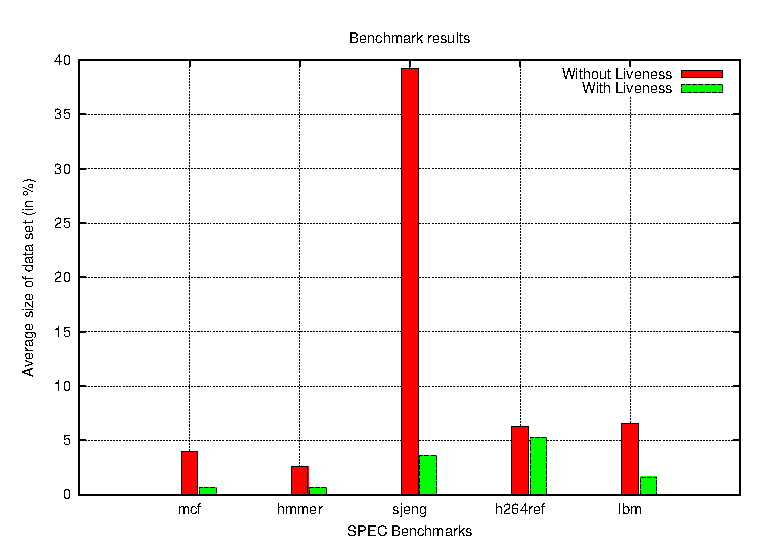
\includegraphics[width = 0.9\textwidth]{./graph.eps}
%     \caption{Percentage reduction in size of data set}
%   \end{figure}
% }
% 
% 
% \frame{
% \frametitle{Limitations of current version of PRISM}
% \begin{itemize}
% \item<1-> PRISM does not perform incremental analysis
% \item<2-> Meet function needs to be explicitly defined in kulang specifications
% \item<2->The meet function can be inferred from the lattice of the data flow problem
% \item<3-> There is no proper way to debug the kulang specifications 
% \item<4-> Hard to understand the specification language
% \end{itemize}
% }
% 
% \part{Future Work}
% \frame{\partpage}
% 
% \frame{
% \frametitle{Future Work}
% \begin{itemize}
% \item<1-> Method to restrict the size of affected region in Constant Propagation
% \item<2-> Incremental analysis in PRISM 
% \item<3-> Simplified Kulang specification
% \end{itemize}
% }

\part{Thank You !}
\frame{\partpage}

\end{document}
